\chapter{Teoría y métodos computacionales}\label{ch:metodos}
\thispagestyle{empty}

\vspace{50pt}

\begin{adjustwidth}{50pt}{50pt}
    TODO: \todo{cambiar este resumen}
    En este capítulo se revisan nociones básicas de mecánica estadística, se 
    introduce la técnica de simulación de dinámica molecular, se presentan los 
    campos de fuerzas utilizados en esta tesis y los observables que se pueden 
    obtener una vez realizadas las simulaciones. Por último se mencionan los 
    softwares que se usaron/implementaron en esta tesis.
\end{adjustwidth}

\clearpage
\newpage
\thispagestyle{empty}
\mbox{}
\newpage

% Copyright (c) 2024, Francisco Fernandez
% License: CC BY-SA 4.0
%   https://github.com/fernandezfran/thesis/blob/main/LICENSE
\section{Técnicas de simulación a distintas escalas}

Dentro de la física, la química y las ciencias de los materiales existen diversas
técnicas computacionales para desarrollar modelos capaces de predecir y entender 
las propiedades de algún sistema en particular. Estos modelos no son más que 
abstracciones matemáticas o lógicas de la realidad que permiten obtener dicha 
información de interés a costa de renunciar a otra \cite{franco2013}. 
En la Figura \ref{fig:escalas} se muestran aplicaciones específicas de 
simulaciones numéricas que cubren distintos intervalos de escalas espaciales y 
temporales. Con respecto a las baterías de litio, se han estudiado distintas
componentes de las mismas con técnicas tales como DFT \cite{he2019}, Dinámica 
molecular \cite{yao2022}, Monte Carlo \cite{mercer2017}, Monte Carlo cinético 
\cite{gavilan2021}, Dinámica mesoescala \cite{ryan2019} y Modelos del continuo
\cite{brosa2022}. En particular, en esta tesis se utilizan las técnicas 
resaltadas con colores en la Figura \ref{fig:escalas} para estudiar distintos 
aspectos de materiales de interés en el área de las baterías de ion-litio.
\begin{figure}[h!]
    \centering
    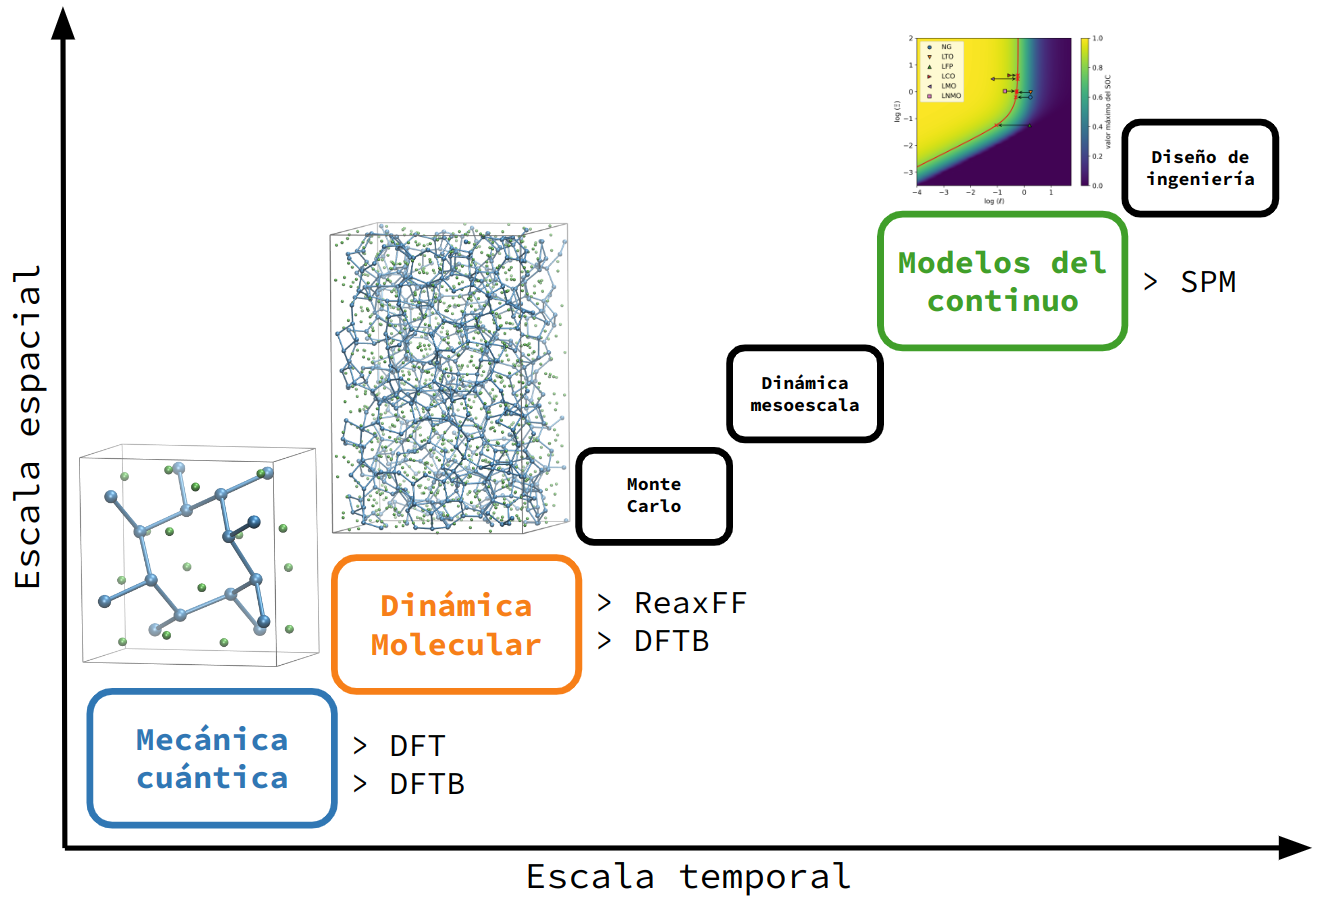
\includegraphics[width=.8\textwidth]{Metodos/tecnicas/escalas.png}
    \caption{Esquema de escalas espaciales y temporales relativas de distintas 
    técnicas de simulaciones computacionales. Se destacan con colores aquellas que 
    se utilizaron en esta tesis mientras que se mencionan otras.}
    \label{fig:escalas}
\end{figure}

Los métodos tradicionales de prueba y error requieren demasiado tiempo como 
para seguir el ritmo rápido de crecimiento en la demanda de sistemas de 
almacenamiento y transporte de energía. %, que actualmente se encuentran limitados por los materiales disponibles. 
Esto ha atraído la atención de investigadores e ingenieros 
hacia el desarrollo de modelos computacionales, desde la escala atómica hasta la 
escala del continuo, y la integración de las mismas, para tener una herramienta 
predictiva para resolver los problemas relacionados a los electrones, los átomos, 
los clusters, las partículas, los electrodos, las celdas e incluso el pack de 
baterías \cite{shi2016}. En particular, en la escala atómica usualmente se tienen
predicciones bajo equilibrio termodinámico de propiedades como la estructura, 
transformaciones de fase, energías de activación, entre otras, como se lo realiza
en la Parte \ref{p:silicio} de esta tesis para el caso de los ánodos de silicio. 
Además de esto, se busca encontrar relaciones que mapeen dichas propiedades con 
descriptores más simples de obtener \cite{juan2021}, como se propone en la Parte
\ref{p:fast-charging} de esta tesis al ajustar datos experimentales con un modelo
del continuo.

Como perspectiva futura, las técnicas de simulación a distintas escalas 
mencionadas aquí pueden combinarse para desarrollar modelos multi-escala 
\cite{franco2019}, y a su vez también pueden aplicarse métodos de inteligencia 
artificial/aprendizaje automático \cite{lombardo2021}, con el objetivo diseñar y 
optimizar las baterías de litio de próxima generación. 


\section{Mecánica cuántica}

El desarrollo de la mecánica cuántica, y las observaciones experimentales que la
validan, fue uno de los avances científicos más significativos del siglo veinte
en describir el universo en el que vivimos \cite{shankar2012}.

La aproxmiación de Born-Oppenheimer permite separar los núcleos de los electrones 
en problemas de mecánica cuántica. Esta aproximación se basa en que los núcleos 
atómicos son mucho más pesados que los electrones individuales. Eso implica que 
puede considerarse que los electrones responden mucho más rápido a los cambios en 
su entorno que los núcleos, lo que permite resolver las ecuaciones que describen 
el movimiento de los electrones para posiciones fijas de los núcleos atómicos. Así 
se encuentra el estado fundamental de los electrones, es decir, la configuración 
de menor energía de los mismos. Esto permite estudiar como varía la energía de los 
materiales con el movimiento de sus átomos.

La ecuación de Schrödinger no-relativista e independiente del tiempo,
\begin{equation}\label{eq:schrodinger}
    H \psi = E \psi,
\end{equation}
caracteriza un sistema físico desde un punto de vista cuántico, donde $\psi$ es un
conjunto de soluciones, o autoestados, del Hamiltoniano $H$ que tienen asociados los
autovalores $E$ que satisfacen dicha ecuación. Para el caso en el que se desee estudiar
la interacción entre varios electrones y núcleos una descripción más completa de la 
ecuación de Schrödinger es la siguiente,
\begin{equation}\label{eq:schrodinger}
    \left[ - \frac{\hbar^2}{2 m} \sum_{i=1}^N \nabla_i^2 + \sum_{i=1}^N V(\mathbf{r}_i) + \sum_{i=1}^N \sum_{i<j} U(\mathbf{r}_i, \mathbf{r}_j) \right] \psi = E \psi,
\end{equation}
donde $\hbar$ es la constante de Plank reducida, $m$ la masa del electrón, el primer 
término describe la energía cinética de cada electrón, el segundo la energía de 
interacción de cada electrón con todos los núcleos y el tercero la energía de 
interacción entre distintos electrones. Este último término es el más crítico desde 
el punto de vista de la resolución de la ecuación.


\subsection{Teoría del funcional de la densidad (DFT)}

La teoría del funcional de la densidad (DFT por sus siglas en inglés
\textit{Density functional theory}) es un método altamente efectivo para 
encontrar soluciones a la ecuación fundamental que describe el comportamiento 
cuántico de átomos y moleculas en sistemas de materia condensada, la ecuación 
\ref{eq:schrodinger} de Schrödinger, en situaciones de utilidad práctica 
\cite{sholl2022}.

\subsection{Funcional de la densidad de enlace estrecho (DFTB)}\label{s:dftb}

\chapter{Software desarrollado}

En la última década, Python se ha convertido en un lenguaje de programación 
importante dentro de la comunidad científica debido a su facilidad de uso y 
versatilidad en la manipulación y visualización de datos ~\cite{millman2011}. 
Por lo tanto, los software diseñados en esta tesis han sido escritos en este
lenguaje y construidos sobre las librerías usuales del cómputo científico como
NumPy \cite{numpy}, SciPy \cite{scipy}, pandas \cite{pandas}, 
matplotlib \cite{matplotlib} y scikit-learn \cite{sklearn1, sklearn2}. 


\section{Control de calidad de software}

El control de calidad del software hace referencia al conjunto de reglas y 
procedimientos que deben utilizarse para verificar que el software cumple 
determinados estándares de calidad subjetivos. Un procedimiento habitual son las 
pruebas unitarias (\textit{unit testing} en inglés), que consisten en aislar una 
función del código y comprobar que funciona como se espera \cite{jazayeri2007}. 
Otro procedimiento habitual se define a partir de este y es el 
\textit{code-coverage}, que determina que proporción del software se ha testeado
\cite{miller1963}. El estilo y la legibilidad del código también es importante
y aquí se ha seguido la guía de estilo PEP8 de Python, la misma se asegura con 
la herramienta flake8. Además, los mismos fueron desarrollados utilizando control 
de versiones git y distribuidos bajo la Licencia MIT, fomentando su uso tanto en 
entornos académicos como comerciales. Todo esto se realizó buscando que el 
software sea fácil de mantener y que respete los estándares de la comunidad Python.


\section{galpynostatic}

Este paquete denominado \path{galpynostatic} fue escrito para la utilización
del modelo heurístico presentado en el capítulo TODO. El mismo distribuye los 
datos de los diagramas galvanostáticos, un módulo de preprocesamiento de datos
para obtener capacidades de descarga a un potencial de corte dado a partir de 
medidas de perfiles galvanostáticos y una clase que realiza la regresión sobre la 
superficie y permite diferentes tipos de gráficos y estimaciones de parámetros.

A continuación se muestra un ejemplo de uso:

\lstinputlisting[language=Python]{apendices/ejemplo_galpynostatic.py}

A \path{galpynostatic} se le realizan múltiples pruebas unitarias sobre datos de
de electrodos actuales y de materiales de investigación de próxima generación en 
baterías de litio, el \textit{coverage} del mismo alcanza el 100\% del software
en su versión inicial.

Por último, el código fuente está disponible en un repositorio público 
(\url{https://github.com/fernandezfran/galpynostatic}) y todos los nuevos cambios 
confirmados en este repositorio se prueban automáticamente con el servicio de 
integración continua de GitHub Actions. También se genera una documentación a 
partir de los docstrings del código, junto con una guía de instalación,
tutoriales y ejemplos con aplicaciones reales, que se hacen públicos en el 
servicio read-the-docs (\url{https://galpynostatic.readthedocs.io/en/latest/}). 
Además, \path{galpynostatic} está disponible para su instalación en el Python 
Package-Index (\url{https://pypi.org/project/galpynostatic/}).

%
%\section{galpynostatic.metric}
%
%TODO
%
%
%\section{macchiato}
%
%TODO
%
%Ejemplo de cálculo del corrimiento químico de la estructura cristalina 
%Li$_{13}$Si$_{4}$ mediante el uso del modelo a primeros vecinos introducido en 
%el capítulo TODO:
%\lstinputlisting[language=Python]{apendices/ejemplo_macchiato.py}
%
%
%\section{Otros códigos}
%
%\subsection{sierras}
%Con \path{sierras} se automatiza el proceso de ajustar la ecuación de Arrhenius 
%(\ref{eq:arrhenius}) en procesos difusivos y la obtención de información a partir 
%de la misma. Este código también se encuentra público 
%(\url{https://github.com/fernandezfran/sierras}) y cada vez que se realiza un 
%cambio se llevan a cabos tests unitarios sobre distintos datos extraídos de 
%literatura. Un ejemplo simple de como se utiliza se presenta a continuación:
%
%\lstinputlisting[language=Python]{apendices/ejemplo_sierras.py}
%
%La versión inicial de este código fue presentada como trabajo final en la materia
%\href{https://github.com/leliel12/diseno_sci_sfw}{\tt Diseño de software para 
%cómputo científico.}
%
%\subsection{exma}
%Para analizar trayectorias de dinámica molecular, dentro de la comunidad de Python
%se encuentra la librería \path{MDAnalysis} \cite{mdanalysis1, mdanalysis2}. Sin
%embargo, no todos los observables descriptos en la sección \ref{s:observables}
%han sido implementados, por ejemplo, no se puede calcular directamente el número
%de coordinación. Para ello se escribió \path{exma}
%(\url{https://github.com/fernandezfran/exma}), que además de contar con esta
%implementación presenta distintas facilidades para computar observables 
%electroquímicos presentados en distintos capítulos de esta tesis. Algunas partes
%de este software han sido escritas en \path{C}, para tener mayor velocidad de 
%cálculo, y tienen una interfaz en Python para ser utilizadas.
%
%\subsection{aelm}
%Para el método de exploración acelerada de mínimos locales, introducido en 
%la sección \ref{s:aelm} del capítulo \ref{ch:caracterizacion}, se escribió un 
%módulo de Python, \path{aelm} (\url{https://github.com/fernandezfran/aelm}), que 
%toma una trayectoria de una dinámica molecular sesgada, minimiza cada uno de los 
%frames con algún programa de dinámica molecular a elección (\path{LAMMPS} o 
%\path{GEMS}, por ejemplo) y guarda las configuraciones atómicas y las energías 
%para su posterior análisis, como se realizó en el capítulo 
%\ref{ch:caracterizacion} ¿o TODO?
%
%\subsection{cluster-connections}
%Se escribió un código en \path{C++}, 
%\url{https://github.com/fernandezfran/cluster-connections}, con un algoritmo de
%\textit{clustering} para deconvolucionar numéricamente el segundo pico de la RDF
%según la cantidad de vecinos que interconectan a segundos vecinos, como se analizó
%en la sección \ref{s:interconexion} del capítulo \ref{ch:caracterizacion}, 
%en la figura \ref{fig:interconexiones}.



\section{Mecánica estadística}

En la mayoría de los experimentos que se realizan en un laboratorio se obtiene 
una serie de mediciones sobre sistemas macroscópicos, usualmente constituidos por 
más de 10$^{20}$ moléculas, durante un período de tiempo, a las cuales luego se 
les realiza un promedio. La mecánica estadística ofrece una interpretación de 
las propiedades del equilibrio de sistemas macroscópicos a partir de una teoría 
molecular aplicada a su configuración microscópica ~\cite{hill1986}.

Esta teoría relaciona el promedio temporal de una variable mecánica con el 
promedio de ensambles, donde un ensamble es una colección de un número muy largo
de sistemas construidos de manera tal que reproducen las propiedades 
termodinámicas del sistema en cuestión a partir de sus configuraciones atómicas
\cite{salinas2001}. Esto es el primer postulado de la Mecánica estadística y se 
lo conoce como la \textit{hipótesis ergódica}: \say{El promedio temporal de una 
variable mecánica $M$ en el sistema termodinámico de interés es igual al promedio 
de ensambles de $M$, en el límite del conjunto de ensambles que tiende a infinito, 
siempre que los sistemas del conjunto de ensambles reproduzcan el estado 
termodinámico y el entorno del sistema real de interés}. Para poder aplicar
este postulado se necesita conocer la probabilidad relativa de cada uno de los 
estados presentes en el ensamble. A esto se refiere el segundo postulado de la 
Mecánica estadística de \textit{igual probabilidad a priori}: \say{En un conjunto 
de ensambles representativo de un sistema termodinámico aislado, los sistemas del 
conjunto de ensambles se distribuyen uniformemente, es decir, con igual 
probabilidad o frecuencia, sobre los posibles estados con los valores
especificados de dicho sistema termodinámico aislado}. En otras palabras, cada 
estado esta representado por la misma cantidad de sistemas en el ensamble.

Cuando las \textit{fluctuaciones} son pequeñas, la función de distribución de 
probabilidad de la variable mecánica $M$ tiene una forma gaussiana en torno a su 
valor medio $\overline{M}$, por lo que su dispersión puede caracterizarse 
completamente por su desviación estándar $\sigma_M$, es decir,
\begin{equation}
    \sigma_M = \sqrt{\overline{(M - \overline{M})^2}}.
\end{equation}
Puede demostrarse que las \textit{fluctuaciones} de la variable mecánica $M$ 
decrecen a medida que aumenta el número de particulas $N$ presentes en el sistema 
de forma proporcional a la inversa de su raíz,
\begin{equation}\label{eq:fluctuaciones}
    \frac{\sigma_M}{\overline{M}} \approx \mathcal{O}(N^{-1/2}).
\end{equation}

\subsection{Dinámica molecular}

En la mayoría de los experimentos que se realizan en un laboratorio se obtiene 
una serie de mediciones sobre sistemas macroscópicos, usualmente constituidos por 
más de 10$^{20}$ moléculas, durante un período de tiempo, a las cuales luego se 
les realiza un promedio. La mecánica estadística ofrece una interpretación de 
las propiedades del equilibrio de sistemas macroscópicos a partir de una teoría 
molecular aplicada a su configuración microscópica ~\cite{hill1986}.

Esta teoría relaciona el promedio temporal de una variable mecánica con el 
promedio de ensambles, donde un ensamble es una colección de un número muy largo
de sistemas construidos de manera tal que reproducen las propiedades 
termodinámicas del sistema en cuestión a partir de sus configuraciones atómicas
\cite{salinas2001}. Esto es el primer postulado de la Mecánica estadística y se 
lo conoce como la \textit{hipótesis ergódica}: \say{El promedio temporal de una 
variable mecánica $M$ en el sistema termodinámico de interés es igual al promedio 
de ensambles de $M$, en el límite del conjunto de ensambles que tiende a infinito, 
siempre que los sistemas del conjunto de ensambles reproduzcan el estado 
termodinámico y el entorno del sistema real de interés}. Para poder aplicar
este postulado se necesita conocer la probabilidad relativa de cada uno de los 
estados presentes en el ensamble. A esto se refiere el segundo postulado de la 
Mecánica estadística de \textit{igual probabilidad a priori}: \say{En un conjunto 
de ensambles representativo de un sistema termodinámico aislado, los sistemas del 
conjunto de ensambles se distribuyen uniformemente, es decir, con igual 
probabilidad o frecuencia, sobre los posibles estados con los valores
especificados de dicho sistema termodinámico aislado}. En otras palabras, cada 
estado está representado por la misma cantidad de sistemas en el ensamble.

Cuando las \textit{fluctuaciones} son pequeñas, la función de distribución de 
probabilidad de la variable mecánica $M$ tiene una forma gaussiana en torno a su 
valor medio $\overline{M}$, por lo que su dispersión puede caracterizarse 
completamente por su desviación estándar $\sigma_M$, es decir,
\begin{equation}
    \sigma_M = \sqrt{\overline{(M - \overline{M})^2}}.
\end{equation}
Puede demostrarse que las \textit{fluctuaciones} de la variable mecánica $M$ 
decrecen a medida que aumenta el número de partículas $N$ presentes en el sistema 
de forma proporcional a la inversa de su raíz,
\begin{equation}\label{eq:fluctuaciones}
    \frac{\sigma_M}{\overline{M}} \approx \mathcal{O}(N^{-1/2}).
\end{equation}

Las simulaciones de Dinámica Molecular (MD, de sus siglas en inglés, 
\textit{Molecular Dynamics}) consideran un sistema clásico de muchos cuerpos 
interactuantes bajo un campo de fuerzas newtoniano para estudiar propiedades de 
equilibrio y transporte. Dada la configuración de $N$ partículas se tiene el 
siguiente sistema de ecuaciones de Newton por resolver
\begin{equation}
    m_i \frac{\partial^2 \mathbf{r}_i}{\partial t^2} = \mathbf{F}_i, \quad i = 1,..., N,
\end{equation}
donde $m_i$ es la masa del átomo $i$, $\mathbf{r}_i$ su posición y $\mathbf{F}_i$
la fuerza. Estas ecuaciones de movimiento son integradas en intervalos de tiempo
pequeños que permiten obtener la evolución temporal del sistema, es decir, su
trayectoria. Ya introducida la mecánica estadística, pueden extraerse propiedades
macroscópicas del sistema en equilibrio al considerar configuraciones microscópicas
representativas a distintos instantes de tiempo de la trayectoria
\cite{allen2017, frenkel2001}.

En la Figura \ref{fig:esquema_md} se muestra un diagrama de flujo de un algoritmo
típico de dinámica molecular para entender el funcionamiento de esta técnica de 
simulación. El mismo está conformado por las siguientes partes:
\begin{figure}[h!]
    \centering
    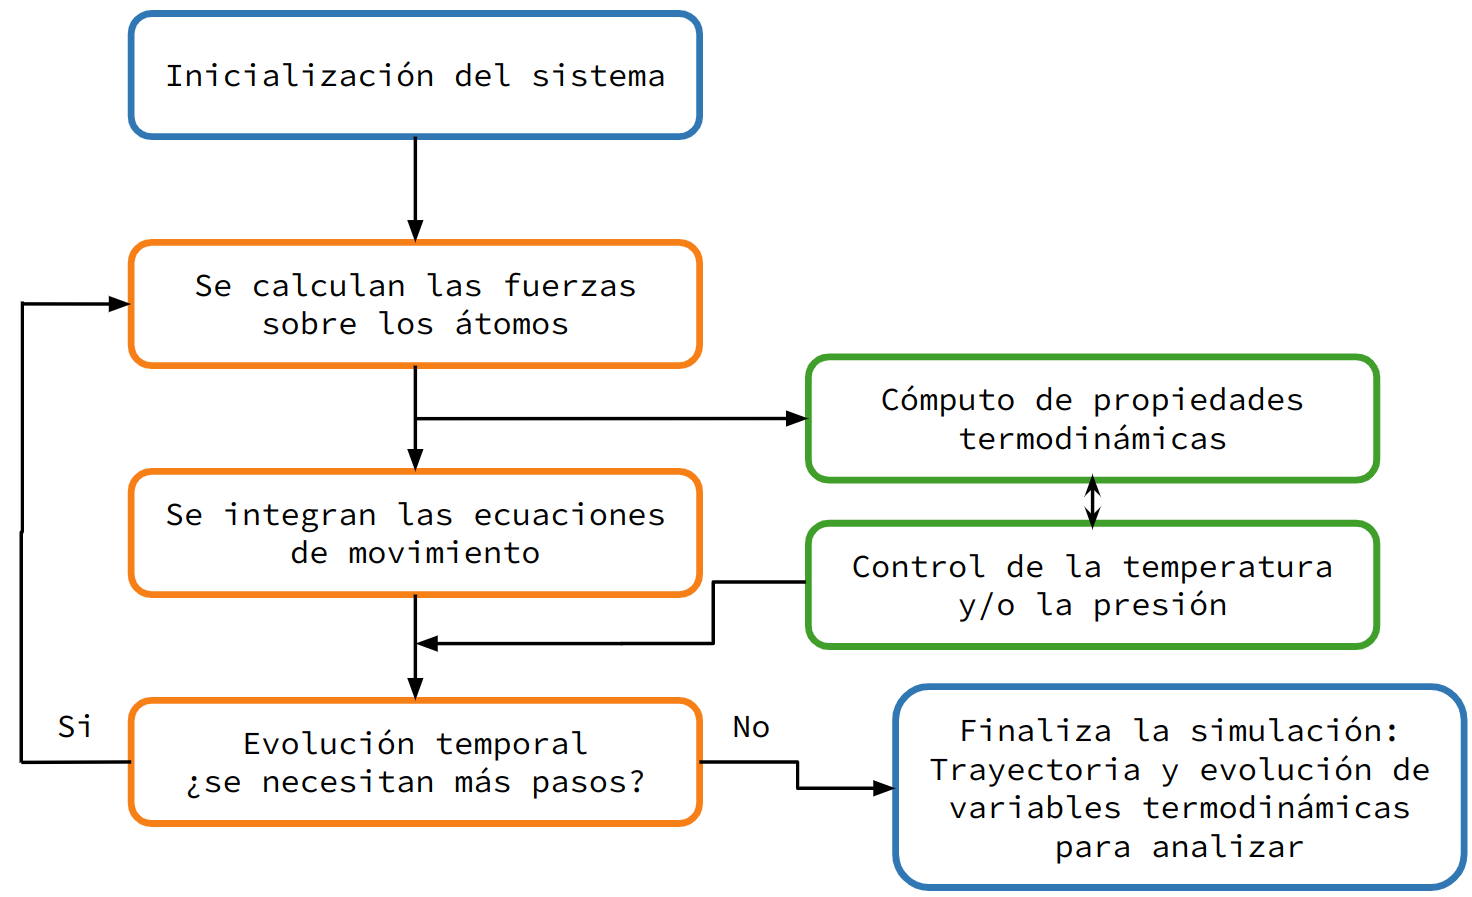
\includegraphics[width=\textwidth]{Metodos/atomicos/esquema.png}
    \caption{Esquema de un diagrama de flujo de una dinámica molecular usual.}
    \label{fig:esquema_md}
\end{figure}
\begin{enumerate}
    \item \textbf{Inicialización del sistema}: se especifican las posiciones y
        velocidades iniciales de los átomos, el tamaño y la forma de la celda de 
        simulación. También se elije un paso temporal y las condiciones de 
        contorno.
    \item \textbf{Campo de fuerzas}: con el sistema inicializado se calcula la 
        fuerza sobre cada uno de los átomos.
    \item \textbf{Cómputo de propiedades termodinámicas}: se realizan los
        cálculos de distintas cantidades de interés, como las energías potencial
        y cinética, la presión y la temperatura, etc.
    \item \textbf{Integración de las ecuaciones de movimiento}: se integran las
        ecuaciones de Newton mediante algún integrador que obtiene las posiciones
        y velocidades del paso temporal siguiente a partir del actual.
    \item \textbf{Control de la temperatura y/o la presión}: para que la 
        simulación se realice en el ensamble termodinámico deseado.
    \item \textbf{Evolución temporal}: se incrementa el tiempo adicionando un
        paso temporal y se vuelve a realizar el cálculo de las fuerzas sobre las 
        nuevas configuraciones hasta alcanzar el número de pasos temporales 
        deseados.
\end{enumerate}
Luego de este proceso se tiene la evolución temporal de las distintas propiedades
termodinámicas de interés y la trayectoria del sistema para ser analizada 
posteriormente, por ejemplo con los observables que se definirán en la sección 
\ref{s:observables}. A continuación se dan más detalles sobre cada uno de los 
pasos mencionados.


\subsubsection{Inicialización del sistema}

Existe una base de datos, Materials Project \cite{materials_project}, 
ampliamente utilizada en el ámbito académico y en la industria que 
recopila estructuras optimizadas con DFT, realiza nuevos cálculos y 
está abierta a la comunidad para su uso y colaboración. Antes de que 
los datos se carguen en la página, los mismos son comparados con resultados 
experimentales para determinar si están dentro de un rango de validez definido. 
En esta tesis en particular, se utilizaron distintas estructuras cristalinas de 
esta base de datos como condiciones iniciales para las posiciones y los tamaños 
de las celdas de simulación.

Las velocidades de los átomos suelen ser generadas de manera aleatoria, a través
de un generador de números pseudo-aleatorio, tomando como argumento una semilla 
para la reproducibilidad de la simulación y una temperatura deseada para el
sistema. Estos números son generados con una distribución gaussiana, donde el 
centro se lo fija a cero para que no haya una velocidad en el centro de masa y 
el ancho está relacionado a la temperatura seleccionada.

Además de dar la configuración inicial de los átomos, es necesario especificar si
los mismos se encuentran dentro de una celda de simulación con un tamaño en
particular para cada una de las direcciones del sistema o si no interactúan fuera
del borde de la estructura que conforman los mismos. En el primero de los casos
se tienen condiciones periódicas de contorno (PBC, por sus siglas en inglés, 
\textit{periodic boundary conditions}), que busca reproducir un sistema infinito,
para que no existan efectos de borde, y consiste en considerar que los átomos se 
encuentran dentro de una celda unidad de una red infinita de celdas idénticas; en
donde si un átomo sale por un extremo de la celda, ingresa por el opuesto. % Una condición que debe cumplir esta celda es que su tamaño en cada una de las direcciones debe ser mayor al radio de corte de las interacciones entre los átomos. Por otro lado, el segundo de los casos es útil considerarlo cuando se tienen nanoestructuras en las cuales los átomos están ordenados de cierta forma que globalmente representan una forma definida y no pueden ser consideradas como una red infinita.


\subsubsection{Campo de fuerzas}

Los potenciales interatómicos empíricos o semi-empíricos que usualmente se 
utilizan en las simulaciones de MD relacionan la fuerza sobre un átomo con el 
entorno del mismo a través de una forma funcional conocida. Existe una gran 
variedad de estos potenciales y la elección de uno de ellos depende del sistema 
de estudio, ya que algunos potenciales representan de mejor manera gases y otros 
metales, por ejemplo. El potencial de Coulomb \cite{coulomb} considera las 
partículas como cargas puntuales que interactúan electrostáticamente. Los 
potenciales de Tersoff \cite{tersoff} o de Stillinger-Weber 
\cite{stillinger-weber} se desarrollaron especialmente para el modelado de 
materiales con enlaces covalentes fuertes. %, como es el caso del carbono o del silicio. 
El método del átomo embebido (EAM, de sus siglas en inglés) \cite{eam} 
y el EAM modificado (MEAM) \cite{meam} están diseñados para simular sistemas 
metálicos. Otros potenciales con enfoques más avanzados permiten simular
reacciones químicas en algunos sistemas, como es el caso de el COMB 
(\textit{charge-optimized many-body}) \cite{comb}, que incorpora una 
equilibración de las cargas en el modelo, o el del ReaxFF (\textit{reactive 
force fields}) \cite{reaxff}, que combina en un solo modelo distintas 
componentes de las que fueron mencionadas. En el último tiempo también se han 
desarrollado potenciales interatómicos de aprendizaje automático 
\cite{behler2016, behler2017, deringer2019}, que no tienen una forma funcional con
una interpretación física, si no más bien un mapeo entre las posiciones y la 
fuerza o la energía de un cálculo de un nivel más complejo, como puede ser DFT.

Para calcular la fuerza que actúa sobre el átomo $i$ se utiliza el opuesto 
de la derivada del potencial,
\begin{equation}\label{eq:fuerzas}
    \mathbf{F}_i = - \frac{\partial V}{\partial \mathbf{r}_i}.
\end{equation}

Para entender el comportamiento de los campos de fuerza se considera como ejemplo 
representativo el potencial de a pares de Lennard-Jones \cite{lennard-jones}, 
debido a que tiene una expresión simple de analizar,
\begin{equation}
    V_{LJ} = 4\varepsilon \left[ \left( \frac{\sigma}{r} \right)^{12} - \left( \frac{\sigma}{r} \right)^{6} \right],
\end{equation}
donde $r$ es la distancia entre dos átomos, $\varepsilon$ indica la profundidad 
del pozo del potencial que se encuentra en $r_m = 2^{1/6} \sigma$ y $\sigma$ es el
radio del átomo. En la figura \ref{fig:lj} se muestra el comportamiento de este
potencial, si la distancia entre dos átomos es menor a $r_m$ entonces se repelen,
si es mayor a dicha distancia, se atraen. Cuando la distancia entre dos átomos es 
infinita, los mismos no interactúan, en el caso práctico se define una distancia 
de corte, conocida como el \textit{radio de corte}, $r_{\text{cut}}$, a partir de 
la cual se considera que el potencial es nulo. Para evitar discontinuidades en 
este punto se suelen utilizar distintas técnicas como el truncado y desplazado o 
se multiplica al potencial alrededor de dicho punto por una función suave, que 
hace que el potencial se iguale suavemente a cero.
\begin{figure}[h!]
    \centering
    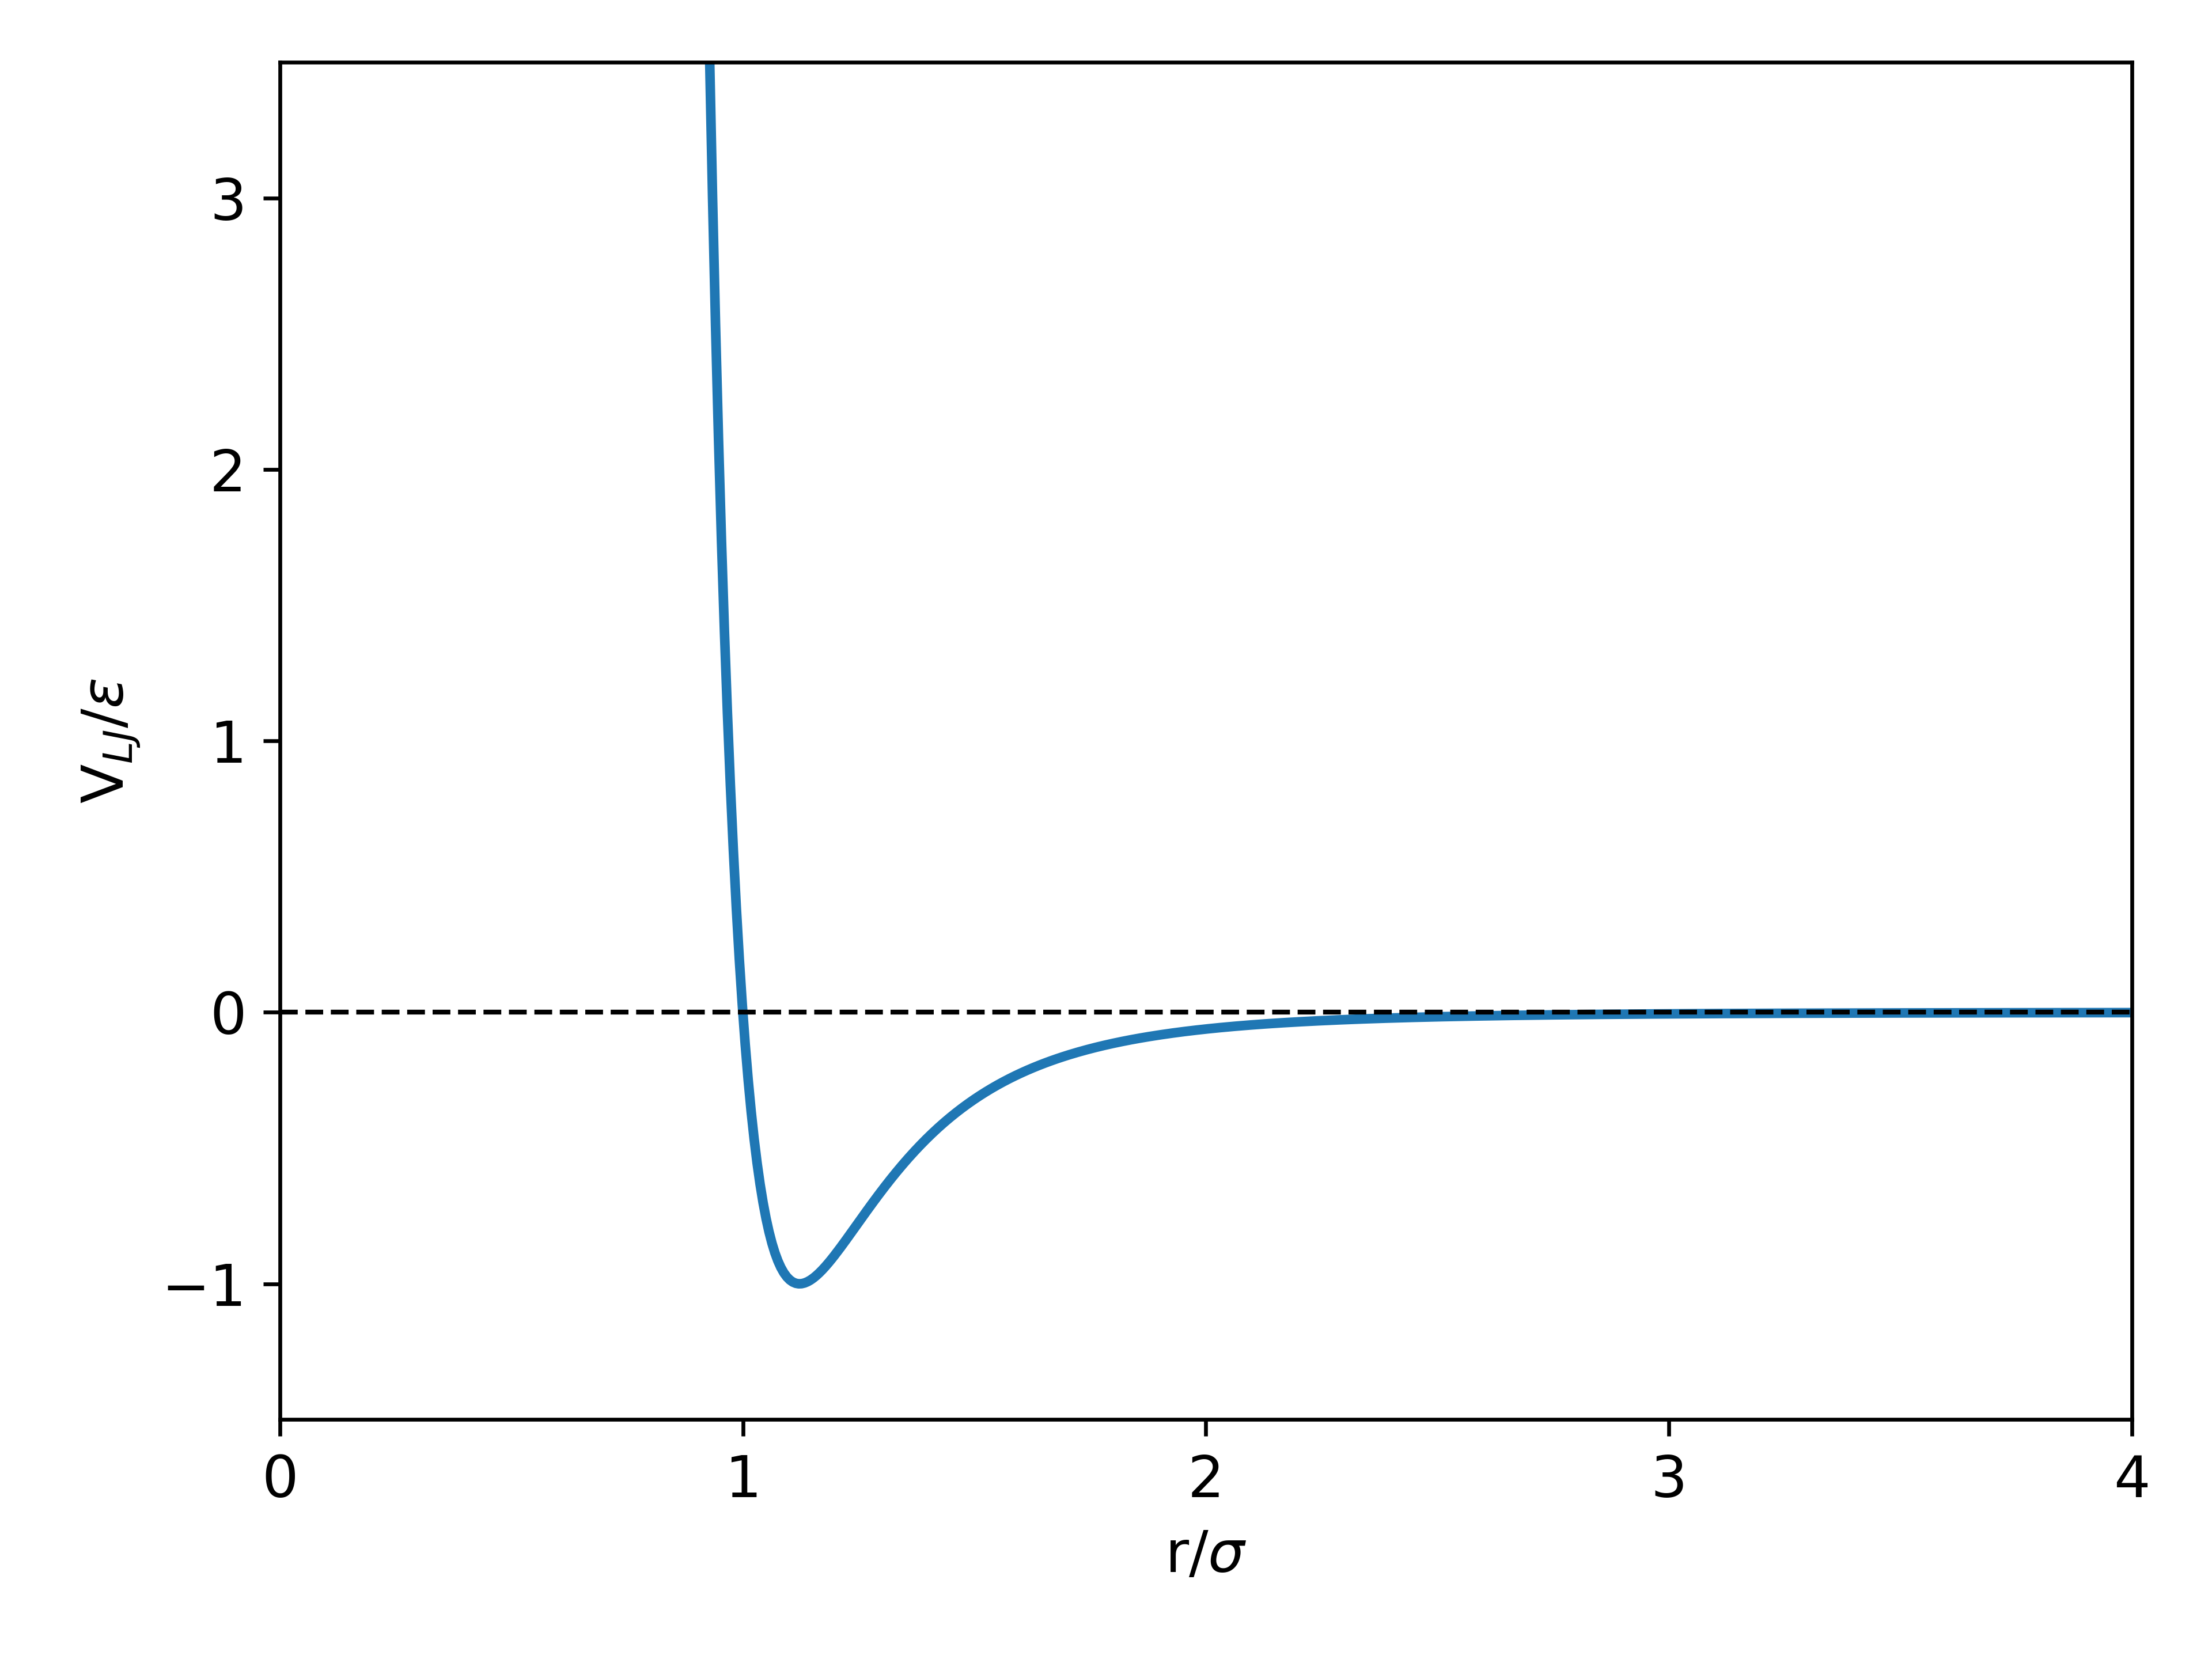
\includegraphics[width=0.7\textwidth]{Metodos/atomicos/lj.png}
    \caption{Gráfico de un potencial de Lennard-Jones en unidades reducidas.}
    \label{fig:lj}
\end{figure}

El ReaxFF \cite{reaxff} es el potencial reactivo del estado del arte para 
utilizar en simulaciones de MD de sistemas de interés en baterías de litio, ya
que representa adecuadamente la asociación y disociación de enlaces de átomos al 
considerar que la energía del sistema, $E_{\text{system}}$, se encuentra dividida
en varias contribuciones de energías parciales,
\begin{equation}\label{eq:reaxff}
    E_{\text{system}} = E_{\text{bond}} + E_{\text{over}} + E_{\text{under}} + E_{\text{val}} + E_{\text{pen}} + E_{\text{tors}} + E_{\text{conj}} + E_{\text{vdWaals}} + E_{\text{Coulomb}}.
\end{equation}
Una de las suposiciones fundamentales del ReaxFF es que el orden de enlace entre
un par de átomos puede obtenerse directamente de la distancia que los separa, 
esto se asegura con el término $E_{\text{bond}}$. $E_{\text{over}}$ y 
$E_{\text{under}}$ se agregan para imponer penalidades a los átomos 
sobrecoordinados o subcoordinados, utilizando la teoría de la valencia del enlace.
$E_{\text{val}}$ considera la contribución a la energía por el ángulo de valencia, 
mientras que $E_{\text{pen}}$ penaliza sistemas para reproducir la estabilidad de 
sistemas con dos dobles enlaces que comparten un átomo en un ángulo de valencia.
Las contribuciones a la energía de los ángulos de torsión y de los efectos de 
conjugación están dados por $E_{\text{tors}}$ y $E_{\text{conj}}$, 
respectivamente. Por último, las interacciones repulsivas a distancias 
interatómicas cortas y las atractivas a distancias largas son incluidas para 
todos los pares de átomos mediante un término de van der Waals, 
$E_{\text{vdWaals}}$, utilizando un potencial de Morse, y uno de Coulomb, 
$E_{\text{Coulomb}}$, donde las cargas de los átomos se aproximan a través de 
un método de equilibración.

La expresión dada en la ecuación \ref{eq:reaxff} implica una gran cantidad de 
parámetros ajustables que se obtienen a partir de cálculos de química cuántica
sobre la disociación de enlaces, reacciones de moléculas pequeñas, energías de 
formación y geometrías de distintos compuestos. Una parametrización ya existente
para el sistema Li-Si \cite{fan2013} se utiliza en el capítulo 
\ref{ch:caracterizacion}.

En los capítulos \ref{ch:modelo} y \ref{ch:prediccion} se utiliza un enfoque 
híbrido que consiste en considerar el hamiltoniano del método DFTB, introducido 
en la sección \ref{s:dftb}, en la ecuación \ref{eq:fuerzas} para calcular las 
fuerzas en una dinámica molecular.


\subsubsection{Cómputo de propiedades termodinámicas}

Una vez que ya se conocen las posiciones, velocidades y fuerzas de todos los 
átomos, se tiene toda la información necesaria para computar distintas cantidades 
de interés. Por ejemplo, para el cálculo de la energía total ($E_{\text{tot}}$) 
se tiene la suma de la contribución potencial ($E_{\text{pot}}$) y de la cinética
($E_{\text{cin}}$),
\begin{equation}
    E_{\text{tot}} = E_{\text{pot}} + E_{\text{cin}}.
\end{equation}
La primera de ellas viene dada por 
\begin{equation}
    E_{\text{pot}} = \sum_{i < j} u(\mathbf{r}_{ij}),
\end{equation}
donde $u(\mathbf{r}_{ij})$ es la contribución proveniente de la interacción 
entre los átomos $i$ y $j$. Por otro lado, la energía cinética puede calcularse a
partir de las velocidades de cada uno de los átomos como
\begin{equation}
    E_{\text{cin}} = \frac{1}{2} \sum_{i=1}^{N} m_i v_i^2, 
\end{equation}
donde $m_i$ es la masa del átomo $i$ y $v_i^2$ el módulo de su velocidad. 

También suele ser de interés obtener el valor de la temperatura y de la presión
del sistema. La temperatura en un paso de la simulación puede calcularse 
utilizando que
\begin{equation}\label{eq:tempvel}
    k_B T = \sum_{i=1}^N \frac{m_i v_i^2}{N_f},
\end{equation}
donde $k_B$ es la constante del Boltzmann y $N_f$ los grados de libertad,
aproximados usualmente por $3N$ para sistemas lo suficientemente grandes. Por 
último, la presión puede calcularse como 
\begin{equation}
P = \rho k_B T + \frac{1}{d \cdot V} \left\langle \sum_{i<j} \mathbf{f}(\mathbf{r}_{ij}) \cdot \mathbf{r}_{ij} \right\rangle,
\end{equation}
donde $\rho$ es la densidad, $d$ la dimensión y $V$ el volumen de la celda de 
simulación. El segundo término es conocido como el virial, donde $\mathbf{r}_{ij}$ 
y $\mathbf{f}(\mathbf{r}_{ij})$ son las distancias y las fuerzas entre los átomos $i$ y $j$.


\subsubsection{Integración de las ecuaciones de movimiento}

Para la integración de las ecuaciones de movimiento se utiliza un integrador que 
cumple con la función de evolucionar las velocidades y las posiciones de los 
átomos una vez que ya se conocen las fuerzas aplicadas sobre cada uno de ellos.
Un integrador estándar, utilizado en esta tesis, es el \textit{velocity Verlet}. 
% El mismo conserva la energía total del sistema si no hay ninguna alteración del ensamble.
Para las posiciones se tiene una actualización de las mismas, a partir
del paso actual, como un desarrollo de Taylor de orden 2,
\begin{equation}
    r(t+dt) = r(t) + v(t) dt + \frac{f(t)}{2m} dt^2,
\end{equation}
donde $dt$ es el paso temporal y $m$ la masa del átomo. Para las velocidades se
tiene
\begin{equation}
    v(t+dt) = v(t) + \frac{f(t+dt)+f(t)}{2m} dt,
\end{equation}
es importante notar que para calcular la velocidad del paso temporal siguiente se
necesita tener computadas las fuerzas anteriores y posteriores, por lo cual
primero se calculan las posiciones y, a partir de ellas, las fuerzas y recién 
luego las velocidades. % Una característica a destacar de este integrador, además de conservar la energía total del sistema, es que soporta una elección de pasos temporales más grandes que integradores anteriores, esto hace que se simule el mismo tiempo real con  menos pasos y por lo tanto menos cómputo de fuerzas, que es la parte computacionalmente más costosa del código.


\subsubsection{Control de la temperatura y/o la presión}

Debido a que la dinámica molecular usual se realiza en un ensamble con el número 
de partículas, el volumen y la energía total constantes (NVE) y la mayoría de los
experimentos con los cuales se pueden comparar resultados se llevan a cabo en 
condiciones de temperatura y/o presión constante, es necesario introducir 
distintos termostatos y barostatos que permitan controlar estos parámetros en las 
simulaciones realizadas. Para modelar el comportamiento directamente de estados
de equilibrio en estos ensambles, se puede modificar la dinámica molecular. % Donde estas modificaciones son meramente de conveniencia computacional y pueden producir desviaciones del movimiento newtoniano real, aunque extremadamente pequeñas.

Desde el punto de vista de la mecánica estadística, a un sistema se le puede 
imponer una temperatura (ensamble NVT) si se lo pone en contacto con un baño 
térmico lo suficientemente grande. En dicho caso la probabilidad de encontrar al 
sistema en un estado de energía viene dada por la distribución de 
Maxwell-Boltzmann,
\begin{equation}\label{eq:mb}
    P(v) = \left( \frac{\beta}{2\pi m} \right)^{3/2} exp(-\beta v^2 / (2m)),
\end{equation}
donde $\beta$ es la energía térmica $k_B T$. Esto quiere decir que la velocidad 
de un átomo no se mantiene constante cuando está en contacto con un baño térmico, 
si no que la misma puede fluctuar y la fluctuación va a depender de dicha 
temperatura de la siguiente forma
\begin{equation}
    \sigma_T^2 = \frac{2}{3 N} \langle T \rangle_{NVT}^2,
\end{equation}
que proviene de calcular el segundo y el cuarto momento de la ecuación 
\ref{eq:mb}.

De manera análoga se puede dejar de suponer al volumen como constante y empezar a
pensar que el mismo es una variable, acoplando el sistema a un pistón para tener
una presión deseada (NPT).

Distintos termostatos y barostatos fueron utilizados durante esta tesis, ellos 
son: el termostato y barostato de Berendsen \cite{berendsen1984}, el termostato 
de Langevin \cite{schneider1978, kroger2005}, el termostato de Nosé-Hoover 
\cite{nose1984a, nose1984b, hoover1985} y el barostato de Parrinello-Rahman
\cite{parrinello-rahman}.



% Copyright (c) 2024, Francisco Fernandez
% License: CC BY-SA 4.0
%   https://github.com/fernandezfran/thesis/blob/main/LICENSE
\section{Modelos del continuo}

A partir de los modelos atomísticos, introducidos en la sección \ref{s:atomicos} desde 
el enfoque de la mecánica cuántica y de la mecánica estadística, se puede obtener
información sobre cómo se comportan los materiales que componen las
distintas partes de las baterías de ion-litio en la nanoescala. Esta información 
tiene una importancia crucial, pero sin embargo suele estar limitada por el tamaño
(unos cientos o miles de átomos) y el tiempo (del orden de los nanosegundos) que 
pueden simular. Como consecuencia de esto, se suelen implementar modelos del 
continuo para estudiar a una escala mayor. En lo que respecta a las baterías de 
ion-litio, estos modelos consideran sus diferentes componentes como un medio 
continuo, en vez de considerar partículas discretas o átomos, lo que permite
manejar escalas espaciales y temporales considerablemente mayores \cite{brosa2022}.

Los modelos de batería de tipo continuo pueden dividirse en dos categoría:
empíricos y basados en física. Los modelos empíricos consisten en ajustar 
incrementalmente ecuaciones y parámetros para encontrar la mejor correspondencia
con datos experimentales, representando así el comportamiento de la batería. 
Como ventaja de estos modelos puede destacarse su velocidad de cómputo y su
conjunto reducido de parámetros, sin embargo no se basan en la física subyacente, 
lo que limita obtener una interpretación de los mecanismos internos de la batería.
En contraste, los modelos basados en física representan los fenómenos físicos 
que gobiernan el comportamiento de la batería y pueden utilizarse para producir 
simulaciones con una precisión mayor, respecto a los empíricos. También existen
modelos híbridos que combinan los mejores aspectos de ambas aproximaciones para 
lograr un compromiso adecuado entre la precisión y la velocidad computacional.

Muchos de los electrodos de intercalación de litio que se investigan en los 
laboratorios o que son incorporados en las baterías comerciales, pueden ser 
simulados con modelos matemáticos complejos que consideran las particularidades 
de cada caso \cite{doyle1995}. Los modelos que poseen un mayor nivel de detalles 
pueden ofrecer una mayor precisión sobre las propiedades 
específicas de un electrodo determinado, pero a su vez pueden dificultar la 
compresión de los aspectos físicos ya que requieren una parametrización detallada, 
lo cual, además de ser una carga a veces innecesaria, dificulta una descripción 
más general del problema. 

% Copyright (c) 2024, Francisco Fernandez
% License: CC BY-SA 4.0
%   https://github.com/fernandezfran/thesis/blob/main/LICENSE
\subsection{Modelo de una sola partícula}\label{s:metodologia}

Los modelos de orden reducido buscan simplificar modelos más complejos pero 
conservar sus capacidades predictivas. Estos pueden mejorar la compresión física 
y proporcionar soluciones precisas a un costo computacional significativamente menor.
Este es el caso de los modelos de una sola partícula (SPM, \textit{single particle 
model}), como el que se utiliza en esta tesis, se supone que todas las partículas
dentro del electrodo se comportan de manera similar, lo que hace que todas puedan ser 
representadas por una sola partícula promedio para reducir la complejidad del 
modelado del continuo. Estos modelos pueden ofrecer predicciones rápidas y precisas 
de materiales de baterías reales, lo que tiene numerosas aplicaciones posibles. Por ejemplo, pueden 
utilizarse como herramientas de diseño para 
%facilitar nuevas arquitecturas de electrodos, celdas y paquetes de baterías, y evaluar su rendimiento, lo cual reduce la necesidad de diseñar prototipos costosos. También pueden ser utilizadas para determinar cuál de los distintos tipos de baterías disponibles en el mercado se adapta mejor a un caso de uso particular.
predecir qué tamaño de partícula debería ser necesario para obtener una dada 
performance del material, como se realiza en la parte \ref{p:fast-charging} de 
esta tesis.

En esta tesis se utiliza un modelo de una sola partícula recientemente propuesto 
\cite{gavilan2023} para construir diagramas galvanostáticos de la capacidad máxima 
alcanzada por una sola partícula en función de dos parámetros adimensionales: uno
cinético,
\begin{equation}\label{eq:xi}
    \Xi = k^0 \sqrt{\frac{t_h}{C_r D}},
\end{equation}
y el otro de difusión finita,
\begin{equation}\label{eq:ele}
    \ell = d \frac{V}{A} \frac{C_r}{D t_h},
\end{equation}
donde $k^0$ es la constante cinética, $D$ el coeficiente de difusión, $V/A$ es la 
proporción volumen/superficie, $d$ es el tamaño característico de la partícula, 
$t_h$ el tiempo de una hora (en las unidades que corresponda) y $C_r$ denota la 
velocidad de carga galvanostática (C-rate), que indica cuántas veces se puede 
cargar o descargar una batería en una hora. Los parámetros de todas las ecuaciones 
que siguen a continuación se presentan en la Tabla \ref{t:params}.
\begin{table}[h!]
    \centering
    \caption{Parámetros involucrados en las ecuaciones del modelo de una sola partícula.}
    \setlength\extrarowheight{2pt}\stackon{%
    \begin{tabular}{l l}
        \toprule
        \textbf{Parámetro} & 
        \textbf{Definición} \\
        \midrule
        $\Xi = k^0 \sqrt{t_h / (C_r D)}$ & Parámetro galvanostático cinético \\
        $\ell = d (V/A) (C_r / (D t_h))$ & Parámetro galvanostático de difusión finita \\
        $D$ & Coeficiente de difusión del Li$^+$ \\
        $t, t_h$ & Tiempo y tiempo para una hora \\
        $C_r$ & velocidad de carga galvanostática (C-rate) \\
        $x, x_s$ & Grado de intercalación en el electrodo y en la interfase \\ 
                 & electrodo/electrolito \\
        $Q, Q_{\max}$ & Capacidad y capacidad máxima \\ 
        SOC & Estado de la Carga, $\text{SOC} = Q / Q_{\max}$ \\ 
        $z$ & Parámetro para establecer la geometría de la partícula: \\
            & plana ($z=1$), cilíndrica ($z=2$) o esférica ($z=3$) \\
        $d$ & Longitud de difusión -- radio de la partícula -- espesor \\ 
            & de la lámina \\
        $r$ & Distancia definida entre 0 y $d$ ($0 \leq r \leq d$) \\
        $V$ & Volumen del material activo \\
        $A$ & Área superficial del electrodo/electrolito \\
        $V / A$ & Proporción volumen/superficie, para la geometría plana toma\\
                & el valor de $d$, cilíndrica ($d/2$) o esférica ($d/3$) \\
        $I_c$, $i_c$ & Corriente y densidad de corriente (constantes) \\
        $k^0$ & Constante cinética \\
        $E$, $E^0$, $E_{\text{off}}$ & Potencial del electrodo de trabajo vs Li/Li$^+$,\\
                                     & potencial de equilibrio y de corte \\
        $\alpha$ & Coeficiente de transferencia de carga \\
        $\rho$ & Densidad del material \\
        $M_r$ & Masa molecular del material \\
        $F$ & Constante de Faraday \\
        $R$ & Constante universal de los gases \\
        $T$ & Temperatura absoluta \\
        \bottomrule
    \end{tabular}
    }{}
    \label{t:params}
\end{table}

En este modelo, el grado de intercalación $x$ en el punto $r$ y a tiempo $t$ se 
obtiene resolviendo numéricamente la ecuación diferencial 1D de Fick \cite{bard-electrochemistry}:
\begin{equation}\label{eq:fick}
    \frac{\partial x}{\partial t} = D \left[ \frac{\partial^2 x}{\partial r^2} + \frac{(z - 1)}{r} \left(\frac{\partial x}{\partial r}\right) \right],
\end{equation}
donde $D$ es el coeficiente de difusión y $z$ depende del tipo de geometría de la 
partícula \cite{vassiliev2016}. La ecuación \ref{eq:fick} puede resolverse 
utilizando el método de Crank-Nicolson mediante diferencias finitas 
\cite{crank-nicolson} con las siguientes condiciones de contorno en la superficie
de la partícula ($r = 0$),
\begin{equation}
    \left(\frac{\partial x}{\partial r}\right)_0 = - \frac{I_c}{F A \frac{\rho}{M_r}D},
\end{equation}
y al centro de la partícula ($r = d$),
\begin{equation}
    \left(\frac{\partial x}{\partial r}\right)_d = 0.
\end{equation}

La condición de corriente constante se fija con la ecuación de Butler-Volmer \cite{bard-electrochemistry}
\begin{equation}\label{eq:bv}
    I_c = F A \frac{\rho}{M_r} k^0 \left\{x_s \exp\left[ \frac{(1-\alpha)F(E-E^0)}{RT} \right] - (1 - x_s) \exp\left[ -\frac{\alpha F (E-E^0)}{RT} \right] \right\}
\end{equation}

El modelo parte de las siguientes suposiciones:
\begin{itemize}
    \item El transporte de carga dentro de la partícula está limitado por el
        movimiento de los iones insertados, es decir que el transporte electrónico
        es rápido.
    \item La difusión de los iones obedece la segunda Ley de Fick 1D para 
        geometría plana, cilíndrica o esférica.
    \item Se ignoran limitaciones en la transferencia de masa en el electrolito, dado que el coeficiente de difusión de Li$^+$ en este medio es del orden de 10$^{-5}$ cm$^2$/s \cite{valoen2005}, es decir, varios órdenes de magnitud mayor que en cualquiera de los materiales analizados.
    \item El coeficiente de difusión, $D$, permanece constante durante todo el 
        proceso de intercalación.
    \item El flujo de iones en el centro de la partícula es cero.
    \item La transferencia de carga en la interfase electrodo/electrolito se 
        describe mediante la ecuación de Butler-Volmer.
    \item La constante cinética, $k^0$, es la misma durante todo el proceso de 
        intercalación.
    \item La resistencia de la celda está dada por un valor constante, 
        $R_{\Omega}$.
    \item Se ignora la interacción entre los iones intercalados.
    \item No se consideran los cambios volumétricos de la partícula durante su 
        carga/descarga.
    \item También se ignoran migraciones de los iones por la presencia de un 
        campo eléctrico y reacciones secundarias.
\end{itemize}
La influencia de la mayoría de estas limitaciones a la hora de obtener la 
capacidad de la partícula se discuten en la referencia \cite{gavilan2023}. 


\subsubsection{Derivación de los parámetros adimensionales}\label{s:derivparam}

En esta sección se derivan los parámetros adimensionales considerando una geometría
plana ($z = 1$ en la ecuación \ref{eq:fick}) y las siguientes condiciones de 
contorno para la ecuación de Fick,
\begin{equation}\label{eq:condcort}
    x(r, 0) = 0 \quad y \quad \left(\frac{\partial x(r, t)}{\partial r}\right)_{r=d} = 0,
\end{equation}
lo que significa que la perturbación a la concentración inicial es nula a tiempo
0 y que no hay flujo de iones en el centro del material, respectivamente. Se 
comienza aplicando una transformada de Laplace,
\begin{equation}\label{eq:laplace}
    \hat{f}(s) = \mathcal{L}[f] = \int_0^{\infty} f(t) e^{-s t} dt,
\end{equation}
al término de la izquierda de la ecuación \ref{eq:fick} de Fick 
\todo{(¿acá faltaría aclarar algo?)}
\begin{equation}
    \mathcal{L}\left[\frac{\partial x(r, t)}{\partial t}\right] = s \hat{x}(r, s)
\end{equation}
y al derecho
\begin{equation}
    \mathcal{L}\left[D \frac{\partial^2 x(r, t)}{\partial r^2}\right] = D \frac{\partial^2 \hat{x}(r, s)}{\partial r^2}.
\end{equation}
Esto lleva a una ecuación diferencial ordinaria (ODE) de segundo orden
\begin{equation}\label{eq:ode}
    \frac{\partial^2 \hat{x}(r, s)}{\partial r^2} - \frac{s}{D} \hat{x}(r, s) = 0,
\end{equation}
donde a las condiciones de contorno de la ecuación \ref{eq:condcort} también es 
necesario aplicarles la transformada de Laplace, pero al ser nula para ambos casos
esto se mantiene. Como la ecuación \ref{eq:ode} es una ODE lineal homogénea con 
coeficientes constantes, su solución general tiene la siguiente forma
\begin{equation}
    \hat{x}(r, s) = a(s) e^{-\sqrt{s/D}r} + b(s) e^{\sqrt{s/D}r}.
\end{equation}
donde $a(s)$ y $b(s)$ son constantes de integración independientes de $r$, para 
la condición de contorno considerada y definiendo la transformada de Laplace del 
flujo ($\hat{J}$) como la derivada de la concentración con respecto a la posición
se puede encontrar que 
\begin{equation}
    b(s) = a(s) e^{-2 \sqrt{s/D} r},
\end{equation}
por lo cual 
\begin{equation}
    \hat{x}(r, s) = \frac{\hat{J}(r, s)}{\sqrt{D s}} \frac{\left\{ e^{-\sqrt{s/D}r} + e^{\sqrt{s/D}(r - 2d)} \right\}}{\left\{ e^{-\sqrt{s/D}r} - e^{\sqrt{s/D}(r - 2d)} \right\}}.
\end{equation}
Si se multiplica y divide por $e^{\sqrt{s/D}d}$ se tiene que
\begin{equation}
    \hat{x}(r, s) = \frac{\hat{J}(r, s)}{\sqrt{Ds}} \coth{[\sqrt{s/D} (d - r)]},
\end{equation}
de donde al aplicar el teorema de convolución 
\footnote{Teorema de convolución:
    \begin{equation}
        \mathcal{L}^{-1} \{\hat{f}(s)\hat{g}(s)\} = \int_0^t f(t - \tau) g(\tau) d\tau
    \end{equation}
    con $f(t) = \mathcal{L}^{-1}\{\hat{f}(s)\}$ y $g(t) = \mathcal{L}^{-1}\{\hat{g(s)}\}$.
    En este caso se consideró $g(\tau) = \mathcal{L}^{-1}\hat{J}(r, s)$
    y $f(\tau) = (1/\sqrt{D}) \mathcal{L}^{-1} \left\{ 1/\sqrt{s} \coth{[\sqrt{s/D}(d-x)]}\right\}$.
} 
se obtiene que
\begin{equation}
    x(r, t) = \int_0^t \frac{1}{d - r} \Theta_3\left(0 \left|\frac{D}{(d-r)^2} (t - \tau)\right.\right) J(r, \tau) d\tau.
\end{equation}
donde $\Theta_3(\nu|x)$ es la función tita \cite{bieniasz2015} dada por la 
siguiente expresión
\begin{equation}
    \Theta_3(\nu|x) = \frac{1}{\sqrt{\pi x}} \sum_{n=-\infty}^{\infty} e^{-\frac{1}{x}(\nu + n)^2}.
\end{equation}
En la frontera $r = 0$, donde la transferencia de carga ocurre se tiene
\begin{equation}\label{eq:rel1}
    x(0, t) = \int_0^t \frac{1}{d} \Theta_3\left(0 \left|\frac{D}{d^2} (t - \tau)\right.\right) J(0, \tau) d\tau,
\end{equation}
por lo que se concluye que la concentración está relacionada con la convolución 
de la corriente en dicha frontera.

Ahora, con el propósito de relacionar la concentración con la corriente ahí, se
utiliza la ecuación de Butler-Volmer (ecuación \ref{eq:bv}) con la definición
$\xi = (nF/RT)(E - E^0)$
\begin{equation}
    \frac{i}{nF} = k^0 \left\{ c_R e^{\alpha_a \xi} + c_O e^{-\alpha_c\xi} \right\},
\end{equation}
donde $c_R$ es la concentración de iones de Li insertados y $c_O$ es la 
concentración de sitios disponibles. Como $c_O = c^0 - c_R$ y suponiendo que 
$\alpha_a + \alpha_c = 1$
\begin{equation}\label{eq:rel2}
    \frac{i}{nF} = k^0 (e^{\alpha_a \xi} + e^{-\alpha_c \xi}) \left\{ c^0 \frac{1}{(1 + e^{-\xi})} - c_O \right\},
\end{equation}
Considerando la desviación de la concentración de la especie oxidada con respecto 
a su valor inicial,
\begin{equation}
    x(r, t) = c(r, t) - c^0,
\end{equation}
se puede reescribir la ecuación \ref{eq:rel1} como
\begin{equation}
    c(0, t) = c^0 + \int_0^t \frac{1}{d} \Theta_3\left(0 \left|\frac{D}{d^2} (t - \tau)\right.\right) J(0, \tau) d\tau,
\end{equation}
que junto a la ecuación \ref{eq:rel2} se la puede utilizar para obtener que 
\cite{aoki1984}
\begin{equation}\label{eq:aoki}
    \frac{i}{nFc^0} = k^0 (e^{\alpha_a \xi} + e^{-\alpha_c \xi}) \left\{ c^0 \frac{1}{(1 + e^{-\xi})} - \frac{d}{D} \int_0^{u=\frac{Dt}{d^2}} \Theta_3\left(0 \left| (u - z)\right.\right) \frac{i}{nFc^0} dz \right\},
\end{equation}
donde se realizó el cambio de variables $z = \frac{D}{d^2}\tau$ y se utilizó la 
relación entre el flujo y la densidad de corriente $J(0, \tau) = \frac{i}{nF}$.

Para demostrar la invariancia de la capacidad con los parámetros 
$\Xi = k^0 \sqrt{t_h / (C_r D)}$ (ecuación \ref{eq:xi}) y 
$\ell = d (V/A) (C_r / (D t_h))$ (ecuación \ref{eq:ele}) se necesita relacionar 
la ocupación con el tiempo y la velocidad de carga galvanostática ($C_r$) con
la corriente. Para esto último se tiene que
\begin{equation}
    I_c = \frac{Q}{t_h} C_r
\end{equation}
y a su vez
\begin{equation}
    x = \frac{t}{t_h} C_r,
\end{equation}
por lo que en condiciones galvanostáticas el tiempo de carga y la ocupación 
están linealmente relacionadas. A su vez, puede obtenerse que
\begin{equation}
    \frac{i_C}{nFc^0} = \frac{V}{A} \frac{C_r}{t_h}.
\end{equation}
Si consideramos esta última ecuación y la corriente constante en la ecuación 
\ref{eq:aoki}
\begin{equation}
    \frac{V}{A} \frac{C_r}{t_h} = k^0 (e^{\alpha_a \xi} + e^{-\alpha_c \xi}) \left\{ \frac{1}{(1 + e^{-\xi})} - \frac{V}{A}\frac{C_r}{t_h}\frac{d}{D} \int_0^{u=\frac{Dt}{d^2}} \Theta_3\left(0 \left| (u - z)\right.\right) dz \right\}.
\end{equation}
Si se define ahora la ecuación \ref{eq:ele}, que para el caso de un plano se tiene
$\ell = \frac{d^2}{D} \left(\frac{C_r}{t_h}\right)$, y se usa que
\begin{equation}
    \int_0^{z=u=\frac{Dt}{d^3}} \Theta_3(0|u-z)dz = \frac{D}{d^2} \frac{t_h}{C_r} \int_0^{x'=x} \Theta_3\left(0\left|\frac{D t_h x}{C_r d^2} - \frac{D t_h x'}{C_r d^2}\right.\right)
\end{equation}
se tiene
\begin{equation}
    d \frac{C_r}{t_h} = k^0 (e^{\alpha_a \xi} + e^{-\alpha_c \xi}) \left\{ \frac{1}{(1 + e^{-\xi})} - \int_0^{x'=x} \Theta_3\left(0 \left| \left(\frac{x}{\ell}- \frac{x}{\ell}\right)\right.\right) dx' \right\}.
\end{equation}
Multiplicando ambos lados de la ecuación por el factor $\sqrt{\frac{t_h}{C_r D}}$
\begin{equation}
    d \frac{C_r}{t_h} \sqrt{\frac{t_h}{C_r D}} = k^0 \sqrt{\frac{t_h}{C_r D}} (e^{\alpha_a \xi} + e^{-\alpha_c \xi}) \left\{ \frac{1}{(1 + e^{-\xi})} - \int_0^{x'=x} \Theta_3\left(0 \left| \left(\frac{x}{\ell}- \frac{x}{\ell}\right)\right.\right) dx' \right\},
\end{equation}
de donde emerge la relación para $\Xi$ (ecuación \ref{eq:xi}) y resulta que las 
soluciones de $x$ en función de $\xi$ sólo dependen de los parámetros $\ell$ y
$\Xi$:
\begin{equation}
    \sqrt{\ell} = \Xi (e^{\alpha_a \xi} + e^{-\alpha_c \xi}) \left\{ \frac{1}{(1 + e^{-\xi})} - \int_0^{x'=x} \Theta_3\left(0 \left| \left(\frac{x}{\ell}- \frac{x}{\ell}\right)\right.\right) dx' \right\}.
\end{equation}



\section{Dinámica molecular}\label{md}

Dentro de lo que son las simulaciones computacionales en física, química y
ciencias de los materiales, existen distintas técnicas para realizar modelados
moleculares numéricos para predecir y entender propiedades macroscópicas a partir
de un conocimiento detallado a escala atómica. Sería conveniente utilizar la 
ecuación de Schrödinger dependiente del tiempo para obtener la mayor precisión 
posible, sin embargo, sólo puede ser resuelta en un tiempo razonable para unos 
pocos átomos. En cierto punto necesitamos realizar aproximaciones, una de las más
utilizadas es la dinámica molecular (MD, de sus siglas en inglés, 
\textit{molecular dynamics}) que considera un sistema de $N$ partículas 
interactuantes en un campo de fuerzas newtoniano. Dada la configuración de los 
átomos se tiene el siguiente sistema de ecuaciones
\begin{equation*}
m_i \frac{\partial^2 \mathbf{r}_i}{\partial t^2} = \mathbf{F}_i, \quad i = 1,..., N,
\end{equation*}
donde $m_i$ es la masa del átomo $i$, $\mathbf{r}_i$ su posición y $\mathbf{F}_i$
la fuerza. Estas ecuaciones de movimiento son integradas en intervalos de tiempo
pequeños que permiten obtener la evolución temporal del sistema, es decir, su
trayectoria. Ya introducida la mecánica estadística, pueden extraerse propiedades
macroscópicas del sistema en equilibro al considerar configuraciones microscópicas
representativas a distintos instantes de tiempo de la trayectoria
~\cite{frenkel2001, allen2017}.

Para entender mejor como trabaja esta técnica de simulación es conveniente ver
cómo funciona su código fuente, un diagrama de flujo del mismo se presenta en 
la figura \ref{fig:esquema_md}, donde cada una de sus partes se amplía en la 
siguiente enumeración:
\begin{enumerate}
    \item \textbf{Inicialización del sistema}: se especifican las posiciones y
        velocidades iniciales de los átomos. También se elije un paso temporal, 
        un radio de corte para las interacciones y las condiciones de contorno que
        se van a respetar a lo largo de la simulación. 
    \item \textbf{Cálculo de fuerzas}: con las posiciones especificadas se
        calcula la fuerza sobre cada uno de los átomos a través del campo de 
        fuerzas elegido.
    \item \textbf{Integración de las ecuaciones de movimiento}: se integran las
        ecuaciones de Newton mediante algún integrador que obtiene las posiciones
        y velocidades del paso temporal siguiente a partir del actual.
    \item \textbf{Cómputo de propiedades termodinámicas}: se realizan los
        cálculos de distintas cantidades de interés, como las energías potencial
        y cinética, la presión y la temperatura, etc.
    \item De ser necesario, se aplica algún \textbf{termostato o barostato}
        para realizar simulaciones en el ensamble termodinámico deseado.
    \item \textbf{Evolución temporal}: se incrementa el tiempo adhiriendo un
        paso temporal y se vuelve a realizar el cálculo de las fuerzas sobre las 
        nuevas configuraciones.
\end{enumerate}

\begin{figure}
    \centering
    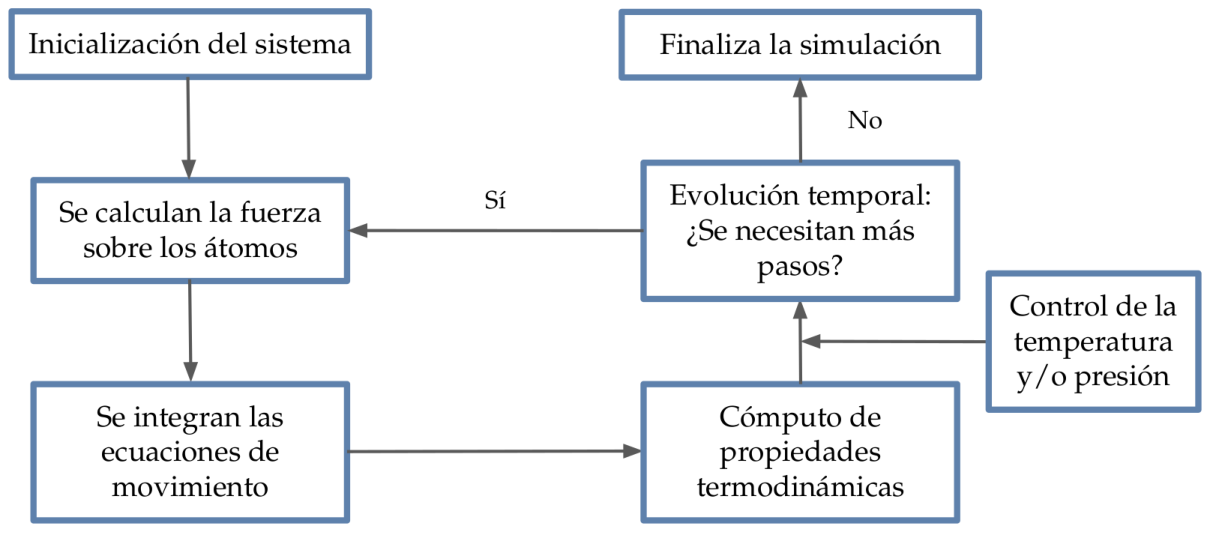
\includegraphics[width=\textwidth]{Metodos/dinamica_molecular/esquema_de_dinamica_molecular.pdf}
    \caption{Esquema de un diagrama de flujo de una dinámica molecular usual.}
    \label{fig:esquema_md}
\end{figure}

\subsection{Configuraciones iniciales}

Si bien las posiciones iniciales de algunos sistemas pueden reproducirse a partir
de los vectores de red de estructuras cristalinas, en otros casos de interés, en 
los cuales hay más de un elemento involucrado, las celdas unidad de mínimos 
locales son más complejas y han sido calculadas y optimizadas mediante la Teoría 
del funcional de la densidad electrónica (DFT, de sus siglas en inglés, density 
functional theory). Realizar estos cálculos suele ser una tarea
computacionalmente costosa y que requiere intervención de científicos 
especializados, para evitar este paso existe una base de datos ampliamente 
utilizada en el ámbito académico y en la industria, Materials Project 
~\cite{materials_project}, que recopila los datos que existen sobre estas 
estructuras cristalinas, realiza nuevos cálculos y está abierta a la comunidad 
para su uso y colaboración. Antes de que los datos se carguen en la página, los 
mismos son comparados con resultados experimentales para determinar si están 
dentro de un rango de validez definido. En esta tesis en particular, fueron 
utilizadas distintas estructuras cristalinas de esta base de datos como 
condiciones iniciales para las posiciones y los tamaños de las celdas de 
simulación.

Las velocidades de los átomos suelen ser generadas de manera aleatoria, a través
de un generador de números pseudo-aleatorio, tomando como argumento una semilla 
para la reproducibilidad de la simulación y una temperatura deseada para el
sistema. Estos números son generados con una distribución gaussiana, donde el 
centro se lo fija a cero para que no haya una velocidad en el centro de masa y 
el ancho está relacionado a la temperatura seleccionada.

\subsection{Condiciones de contorno}

Además de dar la configuración inicial de los átomos, es necesario especificar si
los mismos se encuentran dentro de una celda de simulación con un tamaño en
particular para cada una de las direcciones del sistema o si no interactúan fuera
del borde de la estructura que conforman los mismos. En el primero de los casos
se tienen condiciones periódicas de contorno (PBC, por sus siglas en inglés, 
\textit{periodic boundary conditions}), que busca reproducir un sistema infinito,
para que no existan efectos de borde, y consiste en considerar que los átomos se 
encuentran dentro de una celda unidad de una red infinita de celdas idénticas; en
donde si un átomo sale por un extremo de la celda, ingresa por el opuesto. Una
condición que debe cumplir esta celda es que su tamaño en cada una de las 
direcciones debe ser mayor al radio de corte de las interacciones entre los 
átomos. Por otro lado, el segundo de los casos es útil considerarlo cuando se 
tienen nanoestructuras en las cuales los átomos están ordenados de cierta forma 
que globalmente representan una forma definida y no pueden ser consideradas como
una red infinita.

\subsection{Potenciales interatómicos}

Los potenciales interatómicos empíricos o semi-empíricos que se utilizan en las
dinámicas moleculares relacionan la fuerza sobre un átomo con el entorno químico 
del mismo a través de una forma funcional conocida. Existe una gran 
variedad de estos potenciales y la elección de uno de ellos depende del sistema 
de estudio, ya que algunos potenciales representan de mejor manera gases y otros 
metales, por ejemplo. El potencial de Coulomb ~\cite{coulomb} considera las 
partículas como cargas puntuales que interactúan electrostáticamente. Los 
potenciales de Tersoff ~\cite{tersoff} o de Stillinger-Weber 
~\cite{stillinger-weber} fueron especialmente desarrollados para el modelado de 
materiales con enlaces covalentes fuertes, como es el caso del carbono o del 
silicio. El método del átomo embebido (EAM, de sus siglas en inglés) ~\cite{eam} 
y el EAM modificado (MEAM) ~\cite{meam} están diseñados para simular sistemas 
metálicos. Otros potenciales con enfoques más avanzados permiten simular
reacciones químicas en algunos sistemas, como es el caso de el COMB 
(\textit{charge-optimized many-body}) ~\cite{comb}, que incorpora una 
equilibración de las cargas en el modelo, o el del ReaxFF (\textit{reactive 
force fields}) ~\cite{reaxff}, que combina en un solo modelo distintas componentes
de las que fueron mencionadas.

Uno de los primeros potenciales utilizados en simulaciones computacionales fue 
el potencial interatómico de Lennard-Jones ~\cite{lennard-jones}, que reproduce 
el decaimiento de $r^{-6}$ a distancias largas y viene dado por la siguiente 
expresión
\begin{equation*}
V_{LJ} = 4\varepsilon \left[ \left( \frac{\sigma}{r} \right)^{12} - \left( \frac{\sigma}{r} \right)^{6} \right],
\end{equation*}
donde $r$ es la distancia entre dos átomos, $\varepsilon$ indica la profundidad 
del pozo del potencial que se encuentra en $r_m = 2^{1/6} \sigma$, $\sigma$ es el
radio del átomo. En la figura \ref{fig:lj} 
\begin{figure}
    \centering
    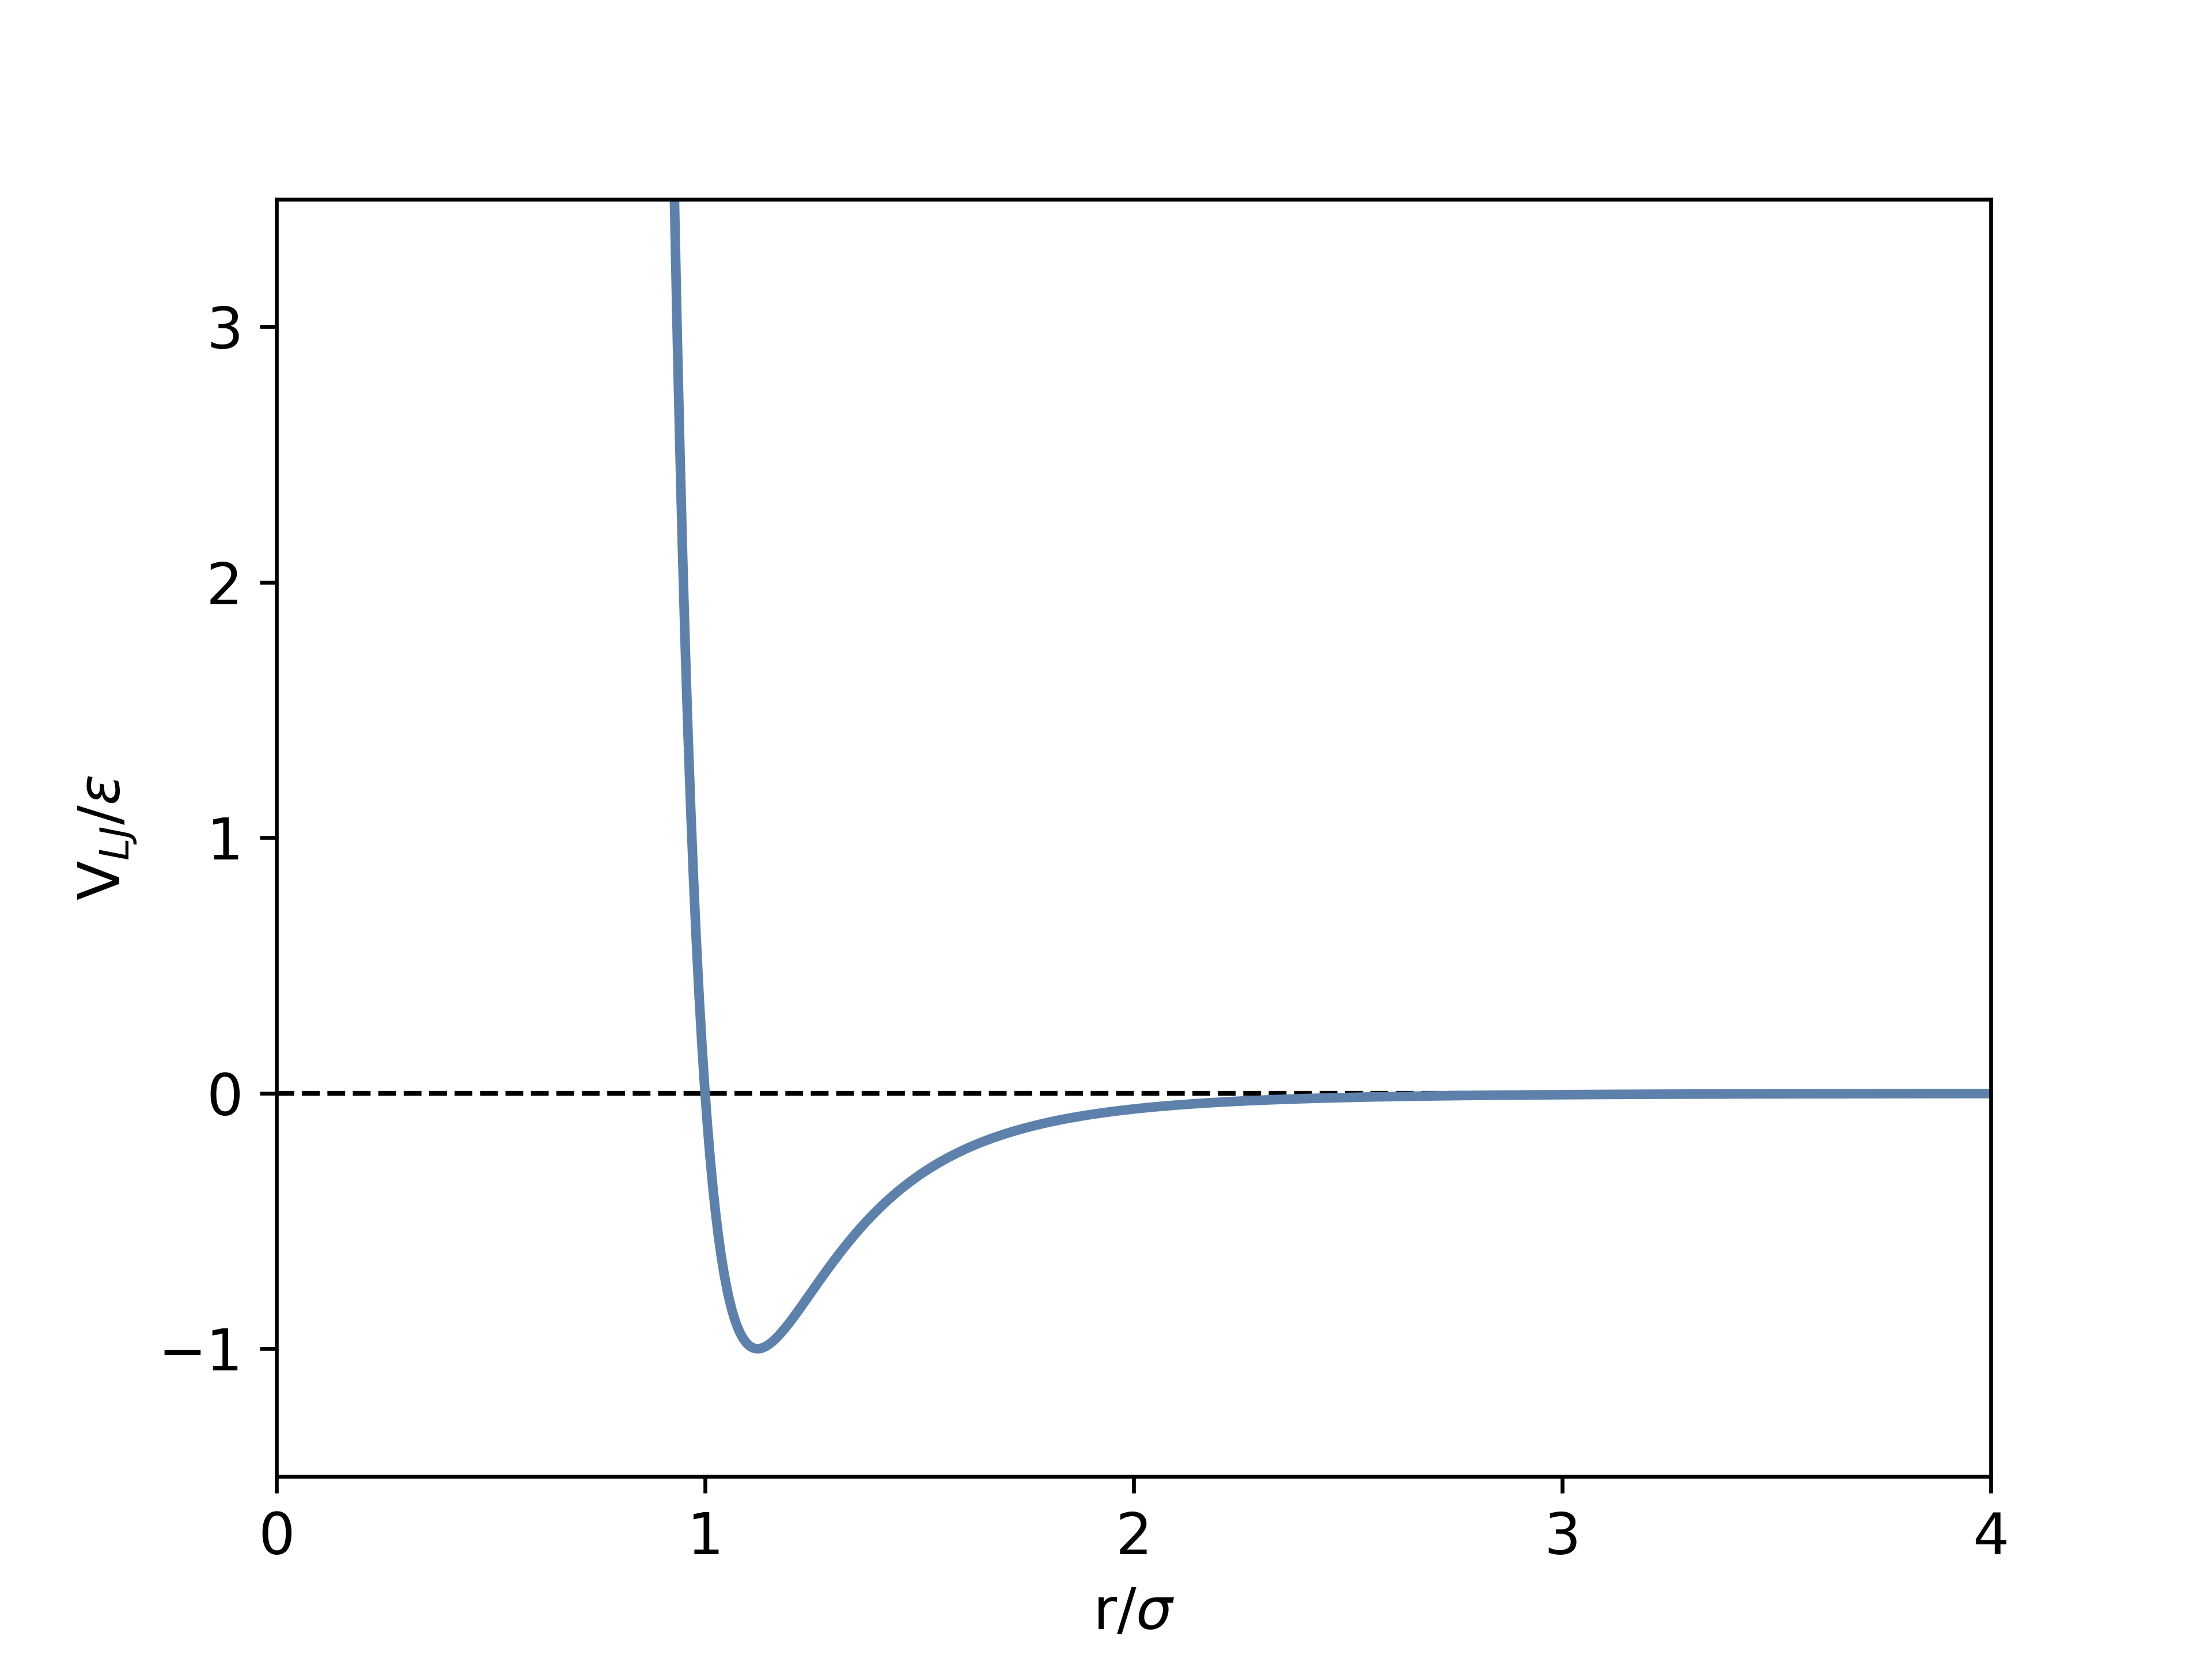
\includegraphics[width=0.7\textwidth]{Metodos/dinamica_molecular/lj.png}
    \caption{Gráfico de un potencial de Lennard-Jones.}
    \label{fig:lj}
\end{figure}
se muestra el comportamiento de este potencial, si la distancia entre dos
átomos es menor a $r_m$ entonces se repelen, si es mayor a dicha distancia, se 
atraen. Cuando la distancia entre dos átomos es infinita, los mismos no 
interactúan, en el caso práctico se define una distancia de corte, conocida como
el \textit{radio de corte}, $r_{cut}$, a partir de la cual se considera que el 
potencial es nulo. Para evitar discontinuidades en este punto se suelen utilizar 
distintas técnicas como el truncado y desplazado o se multiplica al potencial 
alrededor de dicho punto por una función suave, que hace que el potencial se 
iguale suavemente a cero.

Una vez que el potencial interatómico está bien definido, para calcular la fuerza
que actúa sobre el átomo $i$ es necesario computar la fuerza de a pares con todos
los átomos $j$ del sistema. Para esto es necesario calcular las distancias,
considerando la imagen mínima si las condiciones de contorno son PBC, y ver si
las mismas son mayores o menores a $r_{cut}$, si la distancia es mayor entonces
la contribución de esa interacción es igual a cero y si es menor se computa la 
fuerza a través del potencial de la siguiente manera
\begin{equation*}
f_x(r) = - \frac{\partial V(r)}{\partial x}
\end{equation*}
donde $x$ es la componente en alguna de las direcciones definidas para el sistema.

A continuación se presentan dos potenciales interatómicos del estado del arte que
fueron utilizados en esta tesis.

\subsubsection{ReaxFF}\label{s:reaxff}

El campo de fuerza reactivo, ReaxFF ~\cite{reaxff}, representa adecuadamente la
asociación y disociación de enlaces de átomos al considerar que la energía del 
sistema, $E_{system}$, se encuentra dividida en varias contribuciones de energías
parciales,
\begin{equation*}
E_{system} = E_{bond} + E_{over} + E_{under} + E_{val} + E_{pen} + E_{tors} + E_{conj} + E_{vdWaals} + E_{Coulomb}.
\end{equation*}

Una de las suposiciones fundamentales del ReaxFF es que el orden de enlace entre
un par de átomos puede obtenerse directamente de la distancia que los separa, 
esto es asegurado por el término $E_{bond}$.

$E_{over}$ y $E_{under}$ son términos agregados para imponer penalidades a los
átomos sobrecoordinados o subcoordinados, utilizando la teoría de la valencia 
del enlace.

$E_{val}$ considera la contribución a la energía por el ángulo de valencia, 
mientras que $E_{pen}$ penaliza sistemas para reproducir la estabilidad de 
sistemas con dos dobles enlaces que comparten un átomo en un ángulo de valencia.

Las contribuciones a la energía de los ángulos de torsión y de los efectos de 
conjugación están dados por $E_{tors}$ y $E_{conj}$, respectivamente.

Por último, las interacciones repulsivas a distancias interatómicas cortas y 
las atractivas a distancias largas son incluidas para todos los pares de átomos
mediante un término de van der Waals, $E_{vdWaals}$, utilizando un potencial de 
Morse, y uno de Coulomb, donde las cargas de los átomos se aproximan a través de 
un método de equilibración.

Los parámetros ajustables de los potenciales ReaxFF se obtienen a partir de 
cálculos de química cuántica sobre la disociación de enlaces, reacciones de 
moléculas pequeñas, calores de formación y geometrías de distintos compuestos.

\subsubsection{DFTB}

Un método alternativo para obtener las fuerzas en dinámica molecular es a través
de la utilización de un modelo híbrido entre los métodos \textit{ab-initio},
basados en DFT, y el uso de potenciales completamente empíricos, DFTB (de sus 
siglas en inglés, \textit{Density Functional based Tight Binding}), que tiene
la ventaja de ser más transferibles que estos últimos y requiere menos costo
computacional que los primeros.

El método de DFTB se basa en una expansión de segundo orden de la energía total 
de Kohn-Sham ~\cite{dft1, dft2} en la DFT con respecto a las fluctuaciones de la 
densidad de carga. El enfoque de orden cero es equivalente a un esquema estándar 
no auto-consistente (TB), mientras que en el segundo orden se puede derivar una 
expresión transparente, libre de parámetros y fácilmente calculable para los 
elementos matriciales hamiltonianos generalizados. Estos se modifican mediante 
una redistribución auto-consistente de las cargas de Mulliken (SCC).

La energía total de un sistema de $M$ electrones en el campo de $N$ núcleos en
las posiciones $\mathbf{R}$ puede escribirse a través de DFT como
\begin{equation*}
E = \sum_i^{occ} \langle \psi_i | - \frac{\Delta}{2} + V_{ext} + \frac{1}{2} \int' \frac{n(\mathbf{r}')}{|\mathbf{r} - \mathbf{r}'|} | \psi_i \rangle + E_{XC}(n(\mathbf{r})) + \frac{1}{2} \sum_{\alpha, \beta}^N \frac{Z_{\alpha}Z_{\beta}}{|\mathbf{R}_{\alpha} - \mathbf{R}_{\beta}|},
\end{equation*}
donde la primera suma es sobre los autoestados $\psi_i$ ocupados de Kohn-Sham,
$n(\mathbf{r})$ es la densidad electrónica, el segundo término es la contribución
de la correlación de intercambio (XC), y el último término considera la repulsión
de ion-ion. Si se utiliza una densidad de referencia $n_0$ más un término 
pequeño de fluctuación $\delta n$ y se expande $E_{XC}$ a la densidad de 
referencia:
\begin{equation}\label{eq:dft-fluc}
    \begin{aligned}
        E =& \sum_i^{occ} \langle \psi_i | \hat{H}_0 | \psi_i \rangle - \frac{1}{2} \int \int' \frac{n_0' n_0}{|\mathbf{r} - \mathbf{r}'|} + E_{XC}(n_0) - \int V_{XC}(n_0)n_0 + E_{ii} \\
        &+ \frac{1}{2} \int \int' \left(\frac{1}{|\mathbf{r} - \mathbf{r}'|} + \frac{\delta^2 E_{XC}}{\delta n \delta n'}\bigg\rvert_{n_0} \right)
    \end{aligned}
\end{equation}

\begin{enumerate}
    \item \textbf{Enforque de orden cero}

        El método de DFTB de orden cero calcula los elementos de la matriz 
        Hamiltoniana y de solapamiento a partir de una base orbital local con la
        ayuda de DFT-LDA (DFT-\textit{Local density approximation}) y algunas
        aproximaciones en las integrales. Puede verse como una aproximación de 
        una combinación lineal de los orbitales atómicos (LCAO, de sus siglas en 
        ingles, \textit{linear-combination-of-atomic-orbitals}). De esta forma se
        busca evitar las dificultades que surgen a la hora de parametrizar un 
        potencial empírico ~\cite{dftb1, dftb2}.

        En esta aproximación, las ecuaciones de Kohn-Sham son resultas de una
        forma no consistente, ignorando el último término de la ecuación 
        \ref{eq:dft-fluc} y expandiendo los orbitales de Kohn-Sham $\psi_i$ del 
        sistema en términos de las funciones de la base localizadas centradas en 
        el átomo,
        \begin{equation*}
        \psi_i = \sum_{\nu} C_{\nu i} \phi_{\nu}(\mathbf{r}-\mathbf{R}_k),
        \end{equation*}
        resolviendo las ecuaciones de Kohn-Sham para un potencial efectivo de una
        partícula $V_{eff}(\mathbf{r})$,
        \begin{equation}\label{eq:kohn-sham-mod}
            \hat{H}_0 \psi_i(\mathbf{r}) = \varepsilon_i \psi_i(\mathbf{r}), \quad \hat{H}_0 = \hat{T} + V_{eff}(\mathbf{r}),
        \end{equation}
        se tiene como resultado un conjunto de ecuaciones algebraicas,
        \begin{equation}\label{eq:alg-eq}
        \sum_{\nu} C_{\nu i} (H_{\mu \nu} - \varepsilon S_{\mu \nu}) = 0, \quad \forall \mu, i,
        \end{equation}
        donde
        \begin{equation*}
        H_{\mu \nu} = \langle \phi_{\mu}|\hat{H}_0|\phi_{\nu} \rangle, \quad S_{\mu \nu} = \langle\phi_{\mu}|\phi_{\nu}\rangle.
        \end{equation*}

        La energía total del sistema puede ser aproximada como una suma sobre la
        energía de la estructura de bandas y un potencial repulsivo de dos cuerpos
        de corto alcance,
        \begin{equation*}
            \begin{aligned}
                   E_{tot}(\{\mathbf{R}_k\}) &= E_{BS}(\{\mathbf{R}_k\}) + E_{rep}(\{|\mathbf{R}_k - \mathbf{R}_l|\}) \\
                    &= \sum_i n_i \varepsilon_i(\{\mathbf{R}_k\}) + \sum_k \sum_{<l} V_{rep}(|\mathbf{R}_l - \mathbf{R}_k|),
            \end{aligned}
        \end{equation*}
        donde $n_i$ es el número de ocupación del orbital $i$.
        
        Las funciones de onda pseudoatómicas pueden escribirse en términos de los
        orbitales tipo Slater y armónicos esféricos,
        \begin{equation*}
        \phi_{\nu}(\mathbf{r}) = \sum_{n,\alpha,l_{\nu},m_{\nu}} a_{n\alpha} r^{l_{\nu}+n} e^{-\alpha r} Y_{l_{\nu}m_{\nu}}\left(\frac{\mathbf{r}}{r}\right),
        \end{equation*}
        a la hora de realizar una solución auto-consistente a las ecuaciones
        modificadas de Kohn-Sham \ref{eq:kohn-sham-mod}. Estas soluciones son
        utilizadas como funciones de la base LCAO a la hora de tratar el sistema
        sólo considerando los orbitales de valencia.
        
        Como una aproximación, se escribe el potencial de un electrón de una 
        estructura con muchos átomos como una suma de contribuciones atómicas
        esféricas,
        \begin{equation*}
        V_{eff}(\mathbf{r}) = \sum_k V_0^k(|\mathbf{r} - \mathbf{R}_k|),
        \end{equation*}
        donde $V_0$ es el potencial de Kohn-Sham de un pseudo-átomo neutral.

        La matriz de solapamiento consiste solamente de dos elementos centrales
        y puede ser calculada de una forma sencilla
        \begin{equation*}
            H_{\mu\nu}^0 = 
            \begin{cases*}
                \varepsilon_{\mu}^{atomo\ libre} & si $\mu = \nu$ \\
                \langle \phi_{\mu}^{\alpha} | \hat{T} + V_0^{\alpha} + V_0^{\beta} | \phi_{\nu}^{\beta} \rangle & si $\alpha \neq \beta$ \\
                0 & para el resto de los casos,
            \end{cases*}
        \end{equation*}
        donde los índices $\alpha$ y $\beta$ indican el átomo sobre el cual la
        función de onda y el potencial están centrados, sólo dos elementos de la 
        matriz Hamiltoniana son tratados. Debido a que todos los elementos de la 
        matriz dependen sólo de las distancias interatómicas, sólo es necesario
        calcularlos una vez para cada par de tipo de átomo y guardar los valores
        definiendo un ancho de paso. Luego, los elementos para distancias 
        intermedias pueden ser interpolados entre los valores guardados.

        La repulsión a corto alcance $V_{rep}(R)$ puede ser determinada a partir
        de la diferencia en la energía total resultante de un cálculo 
        auto-consistente, $E_{LDA}^{sc}$, y $E_{BS}$ para distintos valores de 
        distancia $R$,
        \begin{equation*}
        V_{rep}(R) = E_{LDA}^{sc}(R) - E_{BS}(R).
        \end{equation*}

        Por último, las fuerzas interatómicas pueden ser derivadas de manera
        explícita para utilizarlas en dinámica molecular de la siguiente forma
        \begin{equation*}
        \mathbf{F}_{\alpha} = - \sum_i n_i \sum_{\mu} \sum_{\nu} C_{\mu i} C_{\nu i} \left(\frac{\partial H_{\mu \nu}^0}{\partial \mathbf{r}_{\alpha}} - \varepsilon \frac{\partial S_{\mu \nu}}{\partial \mathbf{r}_{\alpha}}\right) - \sum_{\beta \neq \alpha} \frac{\partial E_{rep}(|\mathbf{r_{\alpha} - \mathbf{r}_{\beta}|)}}{\partial \mathbf{r}_{\alpha}}.
        \end{equation*}

    \item \textbf{Enfoque de segundo orden}

        En una aproximación de segundo orden se agrega un término, además de
        el usual correspondiente a la \say{estructura de bandas} y el 
        potencial repulsivo de corto alcance, que considera la energía de
        interacción a largo alcance de Coulomb entre las fluctuaciones de la 
        carga a través una redistribución auto-consistente de las cargas de 
        Mulliken (SCC) ~\cite{dftb3}.

        Ahora sí se considera el último término de la ecuación \ref{eq:dft-fluc}
        al descomponer $\delta n(\mathbf{r})$ en contribuciones centradas en el
        átomo, entonces el término de segundo orden queda
        \begin{equation}\label{eq:q1}
        E_{2nd} = \frac{1}{2} \sum_{\alpha, \beta}^N \int \int' \Gamma(\mathbf{r}, \mathbf{r}', n_0) \delta n_{\alpha}(\mathbf{r}) \delta n_{\beta}(\mathbf{r}'),
        \end{equation}
        donde $\Gamma$ denota los coeficiente Hartree y XC. $\delta n_{\alpha}$
        puede ser extendida en una serie de funciones radiales y angulares,
        \begin{equation*}
            \begin{aligned}
                \delta n_{\alpha}(\mathbf{r}) &= \sum_{l,m} K_{ml} F_{ml}^{\alpha}(|\mathbf{r} - \mathbf{R}_{\alpha}|) Y_{lm} \left(\frac{\mathbf{r}-\mathbf{R}_{\alpha}}{|\mathbf{r}-\mathbf{R}_{\alpha}|}\right) \\
                &\approx \Delta q_{\alpha} F_{00}^{\alpha}(|\mathbf{r} - \mathbf{R}_{\alpha}|) Y_{00},
            \end{aligned}
        \end{equation*}
        donde $F_{ml}^{\alpha}$ denota la dependencia radial normalizada de la
        fluctuación de la densidad en el átomo $\alpha$ para el momento angular
        correspondiente. Esta expresión preserva la carga total del sistema.
        Si a la misma se la sustituye en la ecuación \ref{eq:q1},
        \begin{equation*}
        E_{2nd} = \frac{1}{2} \sum_{\alpha,\beta}^N \Delta q_{\alpha} \Delta q_{\beta} \gamma_{\alpha\beta},
        \end{equation*}
        donde
        \begin{equation*}
        \gamma_{\alpha\beta} = \int \int' \Gamma(\mathbf{r},\mathbf{r}',n_0)\frac{F_{00}^{\alpha}(|\mathbf{r} - \mathbf{R}_{\alpha}|)F_{00}^{\beta}(|\mathbf{r} - \mathbf{R}_{\beta}|)}{4 \pi}
        \end{equation*}
        se introduce como abreviatura. En el límite de distancias interatómicas
        grandes, $E_{2nd}$ puede ser vista como una interacción de Coulomb pura
        entre dos cargas puntuales $\Delta q_{\alpha}$ y $\Delta q_{\beta}$. Una
        aproximación simple y muy utilizada en métodos de química cuántica 
        semi-empíricos es aproximar el valor de $\gamma_{\alpha\alpha}$ por la 
        diferencia potencial de ionización atómica y la afinidad electrónica, que
        está relacionada al parámetro de Hubbard $U_{\alpha}$, 
        $\gamma_{\alpha\alpha} \approx U_{\alpha};$ luego, $\gamma_{\alpha\beta}$ 
        sólo depende de la distancia entre los átomos $\alpha$ y $\beta$ y los 
        parámetros $U_{\alpha}$ y $U_{\beta}$, que pueden ser calculados a partir 
        de la segunda derivada de la energía total de un solo átomo con respecto 
        al número de ocupación del último orbital atómico ocupado en LDA-DFT.

        Por último, en este enfoque de segundo orden, la ecuación 
        \ref{eq:dft-fluc} puede escribirse como
        \begin{equation*}
        E_2^{TB} = \sum_i^{occ} \langle \psi_i | \hat{H}_0 | \psi_i \rangle + \frac{1}{2} \sum_{\alpha, \beta}^N \gamma_{\alpha\beta} \Delta q_{\alpha} q_{\beta} + E_{rep}.
        \end{equation*}

        Para estimar las fluctuaciones de la carga se implementa el análisis de
        Mulliken
        \begin{equation*}
        q_{\alpha} = \frac{1}{2} \sum_i^{occ} n_i \sum_{\mu \in \alpha} \sum_{\nu}^N (C_{\mu i}^{*} C_{\nu i} S_{\mu nu} + C_{\nu i}^{*} C_{\mu i} S_{\nu mu})
        \end{equation*}
        y se obtiene un sistema de ecuaciones algebraicas como en la ecuación
        \ref{eq:alg-eq} pero donde el Hamiltoniano ahora considera una 
        corrección debido a la fluctuación de las cargas $H_{\mu \nu}^1$,
        \begin{equation*}
            \begin{aligned}
                H_{\mu \nu} &= \langle \phi_{\mu} | \hat{H}_0 | \phi_{\nu} \rangle + \frac{1}{2}\sum_{\xi}^N (\gamma_{\alpha\xi} + \gamma{\beta\xi}) \Delta q_{\xi} \\
                &= H_{\mu\nu}^0 + H_{\mu\nu}^1, \quad S_{\mu\nu} = \langle \phi_{\mu} | \phi_{\nu} \rangle, \quad \forall \mu \in \alpha, \quad \nu \in \beta.
            \end{aligned}
        \end{equation*}

        En este nuevo enfoque las fuerzas interatómicas para utilizar en 
        simulaciones de dinámica molecular vienen dadas por
        \begin{equation*}
        \mathbf{F}_{\alpha} = - \sum_i^{occ} n_i \sum_{\mu\nu} C_{\mu i} C_{\nu i} \left[\frac{\partial H_{\mu\nu}^0}{\partial \mathbf{r}_{\alpha}} - \left(\varepsilon_i - \frac{H_{\mu\nu}^1}{S_{\mu\nu}}\right) \frac{\partial S_{\mu\nu}}{\partial \mathbf{r}_{\alpha}} \right] - \Delta q_{\alpha} \sum_{\xi}^N \frac{\partial \gamma_{\alpha\xi}}{\partial \mathbf{r}_{\alpha}} \Delta q_{\xi} - \frac{\partial E_{rep}}{\partial \mathbf{r}_{\alpha}}.
        \end{equation*}
 
\end{enumerate}

\subsection{Integrador}

La funcionalidad que cumple un integrador en un código de dinámica molecular es
la de evolucionar las velocidades y las posiciones de los átomos una vez que 
ya se conocen las fuerzas que se aplican sobre cada uno de ellos. Un integrador
estándar, utilizado en esta tesis, fue el \textit{velocity Verlet}. El mismo 
conserva la energía total del sistema si no está siendo aplicado ningún termostato
o barostato que altere el ensamble. Para las posiciones se tiene una
actualización de las mismas, a partir del paso anterior, como un desarrollo de
Taylor
\begin{equation*}
r(t+dt) = r(t) + v(t) dt + \frac{f(t)}{2m} dt^2,
\end{equation*}
donde $dt$ es el paso temporal y $m$ la masa del átomo. Para las velocidades se
tiene
\begin{equation*}
v(t+dt) = v(t) + \frac{f(t+dt)+f(t)}{2m} dt,
\end{equation*}
es importante notar que para calcular la velocidad del paso temporal siguiente se
necesita tener computadas las fuerzas anteriores y posteriores, por lo cual
primero se calculan las posiciones y, a partir de ellas, las fuerzas.

Una característica a destacar de este integrador, además de conservar la energía
total del sistema, es que soporta una elección de pasos temporales más grandes
que integradores anteriores, esto hace que se simule el mismo tiempo real con 
menos pasos y por lo tanto menos cómputo de fuerzas, que es la parte 
computacionalmente más costosa del código.

\subsection{Cómputo de propiedades termodinámicas}

Una vez que ya se conocen las posiciones, velocidades y fuerzas de todos los 
átomos se tiene toda la información necesaria para computar distintas
cantidades de interés, el cómputo de cada una de ellas dependerá del ensamble en
el cual se están realizando las simulaciones.

Las energías que contribuyen a la energía total son dos, la potencial y la
cinética. La primera de ellas viene dada por distintas contribuciones de pares, 
ángulos, enlaces, etc, dependiendo de que tan complejo sea el campo de fuerzas 
utilizado. En el caso de que la interacción sea solo de a pares, la energía 
potencial puede calcularse de la siguiente forma
\begin{equation*}
E_{pot} = \sum_{i < j} u(r_{ij}),
\end{equation*}
donde $u(r_{ij})$ es la contribución proveniente de la interacción entre los 
átomos $i$ y $j$.

Por otro lado, la energía cinética traslacional puede calcularse a partir de las
velocidades de cada uno de los átomos como
\begin{equation*}
E_{cin} = \frac{1}{2} \sum_{i=1}^{N} m_i v_i^2, 
\end{equation*}
donde $m_i$ es la masa del átomo $i$ y $v_i^2$ el módulo de su velocidad. 

También suele ser de interés obtener el valor de la temperatura y de la presión
del sistema. La temperatura en un paso de la simulación puede calcularse 
utilizando que
\begin{equation}\label{eq:tempvel}
    k_B T = \sum_{i=1}^N \frac{m_i v_i^2}{N_f},
\end{equation}
donde $k_B$ es la constante del Boltzmann y $N_f$ los grados de libertad,
aproximados usualmente por $3N$ para sistemas lo suficientemente grandes. Por 
último, la presión puede calcularse como 
\begin{equation*}
P = \rho k_B T + \frac{1}{d V} \left\langle \sum_{i<j} \mathbf{f}(\mathbf{r}_{ij}) \cdot \mathbf{r}_{ij} \right\rangle,
\end{equation*}
donde $\rho$ es la densidad, $d$ la dimensión y $V$ el volumen del sistema. El
segundo término es conocido como el virial, donde $r_{ij}$ y $f(r_{ij})$ son las 
distancias y las fuerzas entre los átomos $i$ y $j$.

\subsection{Termostatos y barostatos}

Debido a que la dinámica molecular usual se realiza en el ensamble NVE y la 
mayoría de los experimentos con los cuales se pueden comparar resultados se 
realizan a temperatura y/o presión constante, es necesario introducir distintos
termostatos y barostatos que permitan controlar estos parámetros en las 
simulaciones realizadas. Para modelar el comportamiento directamente de estados
de equilibrio en estos ensambles, se puede modificar la dinámica molecular. Donde
estas modificaciones son meramente de conveniencia computacional y pueden producir 
desviaciones del movimiento newtoniano real, aunque extremadamente pequeñas.

Desde el punto de vista de la mecánica estadística a un sistema se le puede 
imponer una temperatura si se lo pone en contacto con un baño térmico lo 
suficientemente grande. En dicho caso la probabilidad de encontrar al sistema en
un estado de energía viene dada por la distribución de Maxwell-Boltzmann,
\begin{equation}\label{eq:mb}
P(v) = \left( \frac{\beta}{2\pi m} \right)^{3/2} exp(-\beta v^2 / (2m)),
\end{equation}
donde $\beta$ es la energía térmica $k_BT$. Esto quiere decir que la velocidad de
un átomo no se mantiene constante cuando está en contacto con un baño térmico, si 
no que la misma puede fluctuar y la fluctuación va a depender de dicha temperatura
de la siguiente forma
\begin{equation*}
\sigma_T^2 = \frac{2}{3 N} \langle T \rangle_{NVT}^2,
\end{equation*}
que proviene de calcular el segundo y el cuarto momento de la ecuación \ref{eq:mb}.

De manera análoga puede dejar de pensarse al volumen como constante y empezar a
pensar que el mismo es una variable cuando el sistema está acoplado a un pistón.

Distintos termostatos y barostatos fueron utilizados durante esta tesis, los mismos 
se introducen a continuación.

\subsubsection{MD a temperatura constante: Termostato de Langevin}

Si se considera la ecuación de Langevin \cite{schneider1978}
\begin{equation}\label{eq:langevin}
    m_i \dot{v_i} = F_i - m_i \gamma v_i + R_i(t),
\end{equation}
donde $F_i$ es la fuerza con la que interactúan los átomos entre sí, $\gamma$ la
constante de fricción y $R_i(t)$ es una variable estocástica con media cero 
y que cumple
\begin{equation*}
\left\langle R_i(t) R_j(t+t') \right\rangle = 2m_i \gamma_i k_B T \delta(t') \delta_{ij}.
\end{equation*}
Para aplicar este termostato, y simular a temperatura constante, en conjunto con 
el integrador \textit{velocity Verlet} se tienen que considerar tres parametros
\cite{kroger2005} a la hora de actualizar las velocidades y las posiciones como
\begin{equation*}
a = \frac{2 - \xi dt}{2 + \xi dt},
\end{equation*}
\begin{equation*}
b= \sqrt{k_B T_0 \xi \frac{dt}{2}},
\end{equation*}
\begin{equation*}
c= \frac{2 dt}{2 + \xi dt}
\end{equation*}
donde $\xi$ es el factor de fricción, es decir, con qué intensidad interacciona 
el sistema con el baño térmico. Se tiene entonces una actualización se la siguiente
manera
\begin{equation*}
v(t+dt) = a v(t) + b \eta + \frac{f(t+dt)+f(t)}{2m} dt,
\end{equation*}
\begin{equation*}
r(t+dt) = r(t) + c v(t) dt
\end{equation*}
donde $\eta$ es una distribución gaussiana de números aleatorios con media 0 y
varianza 1. 

\subsubsection{MD a temperatura y/o presión constante: Termostato y Barostato 
de Berendsen}

El termostato de Berendsen \cite{berendsen1984} puede derivarse si se considera 
la ecuación \ref{eq:langevin} sin el término estocástico y se hace una elección
en particular de la constante de fricción. Dicha ecuación de movimiento modificada
representa un escaleo de velocidades, 
\begin{equation*}
v(t) = \lambda v(t),
\end{equation*}
por paso temporal, donde
\begin{equation*}
\lambda = \sqrt{1 + \frac{dt}{\tau_T} \left( \frac{T_0}{T} - 1 \right)}
\end{equation*}
produce un cambio de temperatura igual a
\begin{equation*}
\frac{dT}{dt} = \frac{1}{\tau_T} (T_0 - T)
\end{equation*}
donde $T_0$ es la temperatura de referencia y  $\tau_T$ es la constante de
acoplamiento con el baño térmico y tiene las mismas unidades que el paso temporal.

Para considerar un acoplamiento con un baño de presión contante, Berendsen 
\cite{berendsen1984} agrega un término extra a las ecuaciones de movimiento que
consideran el cambio de presión
\begin{equation*}
\frac{dP}{dt} = \frac{P_0 - P}{\tau_P},
\end{equation*}
donde $P_0$ es la presión de referencia, $P$ la instantánea y $\tau_P$ la 
constante de acoplamiento. Este comportamiento puede producirse si se realiza un
cambio en el virial, escaleando las distancias entre las partículas. Si el 
volumen ahora cambia como 
\begin{equation*}
\frac{dV}{dt} = 3 \alpha V,
\end{equation*}
y se usa que
\begin{equation*}
\frac{dP}{dt} = - \frac{1}{\beta V} \frac{dV}{dt} = -\frac{3\alpha}{\beta},
\end{equation*}
donde $\beta$ es la compresibilidad isotérmica y $\alpha = - \beta (P_0 - P) / (3 \tau_P)$.
Por lo cual las posiciones de los átomos dentro de la caja de simulación en cada
dirección pueden escalearse como
\begin{equation*}
x = \mu x,
\end{equation*}
donde
\begin{equation*}
\mu = \sqrt[3]{1 - \frac{dt}{\tau_P} (P_0 - P)}.
\end{equation*}

\subsubsection{MD a temperatura constante: Termostato de Nosé-Hoover}

Debido a que la temperatura es proporcional al promedio de las velocidades al 
cuadrado, como puede verse en la ecuación \ref{eq:tempvel}, es posible variar
la temperatura al ajustar la razón a la cual el tiempo progresa 
~\cite{nose1984a}. Por lo cual puede introducirse una nueva variable dinámica
$s$ en el Lagrangiano que reescalee la unidad de tiempo, y se añaden términos 
adicionales para obtener el comportamiento deseado ~\cite{rapaport2004}. Lo que 
que provoca que haya dos variables temporales distintas: el tiempo real, o físico, 
$t'$, y un tiempo escalado, o virtual, $t$; que están relacionados a través de 
sus diferenciales,
\begin{equation*}
dt = s(t') dt'.
\end{equation*}
El Lagrangiano de este sistema extendido se escribe como
\begin{equation*}
\mathcal{L} = \frac{1}{2} m s^2 \sum_i \dot{\mathbf{r}}_i^2 - \sum_{i<j} u(\mathbf{r}_{ij}) + \frac{1}{2} M_s \dot{s}^2 - n_f T \log s,
\end{equation*}
donde $T$ es la temperatura deseada, $n_f = 3N_m + 1$ el número de grados de 
libertad, $M_s$ es una masa que se necesita para construir la ecuación de 
movimiento de la nueva \say{coordenada} $s$ y el punto representa la derivada
con respecto al tiempo virtual. Las ecuaciones de movimiento de Lagrange pueden 
obtenerse de la forma usual y son
\begin{equation*}
\ddot{\mathbf{r}}_i = \frac{1}{m s^2} \mathbf{f}_i - \frac{2 \dot{s}}{s} \dot{\mathbf{r}}_i
\end{equation*}
\begin{equation*}
M_s \ddot{s} = m s \sum_i \dot{\mathbf{r}}_i^2 - \frac{n_f T}{s}
\end{equation*}

Ya que la relación entre t y t' depende de toda la historia del sistema, es decir,
\begin{equation*}
t = \int s(t') dt'
\end{equation*}
es más conveniente si las ecuaciones se transforman a las unidades del tiempo
físico ~\cite{nose1984b, hoover1985}, ahora el punto pasa a representar la 
derivada con respecto al tiempo real, y las ecuaciones de movimiento pueden 
reescribirse como
\begin{equation*}
\ddot{\mathbf{r}}_i = \frac{1}{m} \mathbf{f}_i - \frac{\dot{s}}{s} \dot{\mathbf{r}}_i
\end{equation*}
\begin{equation*}
\ddot{s} = \frac{\dot{s}^2}{s} + \frac{G_1 s}{M_s} 
\end{equation*}
donde $G_1 = m \sum_i \dot{\mathbf{r}}_i^2 - n_f T$. La primera de estas 
ecuaciones de movimiento se asemeja a la ecuación newtoniana convencional con un 
término adicional similar al de la fricción, aunque no se trata de una fricción 
verdadera ya que el coeficiente puede ser de cualquier signo. La segunda ecuación 
define el mecanismo de retroalimentación por el que $s$ varía para regular la 
temperatura.

Si se integra la función partición microcanónica del sistema extendido sobre la
variable $s$ se obtiene la función de partición canónica, lo cual demuestra que
los promedios de equilibrio del sistema físico son los del ensamble canónico a
temperatura $T$ ~\cite{nose1984a}. Sin embargo, la temperatura en sí no es 
constante, pero la retroalimentación negativa que actúa a través de $s$ garantiza
que las fluctuaciones sean limitadas y el valor medio sea igual a $T$.

El Hamiltoniano del sistema extendido
\begin{equation*}
\mathcal{H} = \frac{1}{2} m \sum_i \dot{\mathbf{r}}_i^2 + \sum_{i<j} u(\mathbf{r}_{ij}) + \frac{1}{2} M_s \left(\frac{\dot{s}}{s}\right)^2 + n_f T \log s
\end{equation*}
se conserva debido a que no hay fuerzas externas que dependan del tiempo, lo cual 
proporciona una comprobación útil de la precisión de la solución numérica. El 
Hamiltoniano no tiene significado físico, sus dos primeros términos representan 
la energía del sistema físico, pero su suma es libre de fluctuar.

La $M_s$ no tiene ningún significado físico en particular, simplemente es una 
parte de la técnica computacional de cálculo y su valor debe determinarse 
empíricamente, que, en principio, no afecta a los resultados de equilibrio final, 
pero sí influye en su precisión y confiabilidad. Para variaciones pequeñas de $s$, 
el período característico de las fluctuaciones es ~\cite{nose1984a}
\begin{equation*}
\tau_s = 2 \pi \sqrt{\frac{M_s \langle s \rangle^2}{2 n_f T}}
\end{equation*}
y la simulación debe extenderse a lo largo de muchos de estos períodos para evitar 
que estas fluctuaciones influyan negativamente en los resultados.

De una manera similar a la realizada en el algoritmo de Nosé-Hoover para el 
control de la temperatura, el algoritmo de \textbf{Parrinello-Rahman} permite
obtener una representación correcta del ensamble isotérmico-isobárico al 
realizar un \textbf{control de la presión}, donde se permite una evolución 
temporal del volumen de la caja ~\cite{parrinello-rahman}.


\subsection{Observables}\label{s:observables}

Existen distintos observables que pueden calcularse a partir de las posiciones o
de las velocidades a lo largo de una trayectoria proveniente de una dinámica 
molecular, algunos de ellos dan información de carácter estructural, como puede 
ser la distribución radial de a pares, y otros de dinámico, como el 
desplazamiento cuadrático medio que puede ser utilizado para estimar 
coeficientes de difusión.

\subsubsection{Distribución radial de a pares}

La función de distribución radial de a pares (RDF, de sus siglas en inglés
\textit{radial distribution function}), usualmente referida como $g(r)$, permite 
caracterizar la estructura local de un fluido describiendo la probabilidad de 
encontrar un átomo en una cáscara a una distancia $r$ de un átomo de referencia,
\begin{equation*}
g(r) = \frac{V}{N^2} \left\langle \sum_{i=1, i\neq j}^N \delta(\vec{r} - \vec{r}_{ij}) \right\rangle,
\end{equation*}
donde $\langle \cdot \rangle$ indica el promedio temporal, $V$ el volumen, $N$ el
número de partículas y $\vec{r}_{ij}$ la distancia entra la partícula $i$ y la $j$.
Esta cantidad puede calcularse como la razón entre la densidad media $\rho$ a
una distancia $r$ del átomo de referencia y la densidad a esa misma distancia de 
un gas ideal.

Una característica importante de la RDF es que si sus picos están bien definidos
entonces la estructura se corresponde con un sólido, si sus picos están ensanchados
con respecto a estos y, a medida que la distancia aumenta, la $g(r)$ empieza a 
oscilar alrededor de la unidad, entonces se corresponde con un liquido.

\subsubsection{Número de coordinación}

El número de coordinación (CN, de sus siglás en inglés, \textit{coordination 
number}), también llamado ligancia, de un átomo dado en un sistema químico, se 
define como el número de átomos, moléculas o iones unidos a él. Para definirlo 
pueden tomarse dos alternativas, la primera de ellas contando el número de 
vecinos que rodean a un determinado tipo de átomo en promedio hasta un cierto
radio de corte $r_e$, definido por el mínimo en la RDF después de su primer 
pico; la segunda de ellas a partir de la integral de la RDF,
\begin{equation*}
\int_0^{r_e} g(r) dV.
\end{equation*}
De manera análoga pueden definirse el número de coordinación para segundos 
vecinos y así sucesivamente.

\subsubsection{Difusión}

Si una partícula permanece en un sitio por un periodo de tiempo lo suficientemente 
largo, comparado al tiempo que demora en dar un salto hacia otro sitio, entonces 
pierde memoria de donde vino y el próximo salto se dará hacia una dirección 
aleatoria, se dice entonces que el movimiento de la partícula es estocástico y 
que sigue una caminata aleatoria. Si esto se cumple, entonces, el desplazamiento 
cuadrático medio es proporcional al tiempo, donde la constante de proporcionalidad 
es el coeficiente de difusión de traza
\begin{equation}
    D^{*} = \frac{\langle \Delta r^2 \rangle}{2d\cdot t},
\end{equation}
donde $d$ es la dimensión del problema, $t$ el tiempo y 
$\langle \Delta r^2 \rangle$ el desplazamiento cuadrático medio, que en un sistema 
de $N$ partículas puede calcularse de la siguiente manera
\begin{equation*}
\langle \Delta r^2 \rangle = \frac{1}{N} \sum_{i=1}^{N} \langle |\vec{r_i}(t) - \vec{r_i}(t_0)|^2 \rangle.
\end{equation*}

Si se conoce el coeficiente de difusión de traza, entonces el coeficiente de 
difusión químico puede obtenerse de la siguiente relación ~\cite{gomer1990}
\begin{equation}
    D = \left( \frac{\partial (\mu / k_BT)}{\partial ln \theta} \right)_T D^{*},
\end{equation}
donde $\mu$ es el potencial químico y $\theta$ es la concentración.

Usualmente, el tiempo que demora un átomo en dar un salto en una dinámica 
molecular a temperatura ambiente es muy largo, lo que impide tener una buena 
estadística en un tiempo de simulación razonable, por lo que es usual calcular 
el desplazamiento cuadrático medio a distintas temperaturas altas y extrapolar
el valor que se obtendría a temperatura ambiente mediante una ecuación de tipo 
Arrhenius, en la cual el coeficiente de difusión puede separarse en un 
prefactor $D_0$ y un término tipo Boltzmann,
\begin{equation}\label{eq:arrhenius}
D = D_0 e^{-E / k_BT},
\end{equation}
donde $E$ es la energía de activación del proceso. 

